\documentclass{ccnudoc}

\usepackage{multirow, xeCJKfntef, xpinyin}
\usepackage{graphicx}
\usepackage{tabularray}
\usepackage[
  backend = biber,
  style = gb7714-2015
]{biblatex}
\addbibresource{CCNUthesis.bib}
\graphicspath{{figures}}

\hypersetup{
  pdftitle  = {CCNUthesis: 华中师范大学学位论文模版},
  pdfauthor = {夏康玮}
}
% 全角标点放在引号中,需要改成半角式,否则间距过大,不好看
\def\FSID{“{\xeCJKsetup{PunctStyle=banjiao}。}”} % U+3002
\def\FSFW{“{\xeCJKsetup{PunctStyle=banjiao}.}”} % U+FF0E
\def\COFW{“{\xeCJKsetup{PunctStyle=banjiao}:}”} % U+FF1A
\def\SCFW{“{\xeCJKsetup{PunctStyle=banjiao};}”} % U+FF1B


\title{\textcolor{MaterialIndigo800}{%
  \textbf{CCNUthesis: 华中师范大学学位论文\xpinyin[font=\sffamily,format=\color{MaterialIndigo800}]{模}{mu2}板}}}
\author{夏康玮}
\date{\DocDate \quad \DocVersion%
  \thanks{%
    \parbox{0.5\textwidth}{
      \url{https://github.com/xkwxdyy/CCNUthesis} \\
      \url{https://gitee.com/xkwxdyy/CCNUthesis}
    }
  }
}


\begin{document}
\newgeometry{
  left   = 2.2 in,
  right  = 1.25 in,
  top    = 1.25 in,
  bottom = 1.00 in
}

\maketitle

% !TeX root = ../CCNUthesis.tex

\begin{abstract}
  华中师范大学学位论文 \LaTeX{} 模板 \cls{CCNUthesis} 基于本科生院的论文撰写规范制作,同时参考研究生院提供的《研究生学位论文规范》,用于生成符合华中师范大学学位论文排版要求和相应的国家规范、行业标准的学位论文,旨在为同学提供毕业论文书写的方便。
\end{abstract}

\def\abstractname{Abstract}
\begin{abstract}
The \cls{CCNUthesis} class is intended for typesetting Central China Normal University dissertations with \LaTeX{}, providing support for bachelor, master, and doctoral thesis.
\end{abstract}

\vspace{2cm}
\def\abstractname{特别声明}
\begin{abstract}
在使用本模板时,我们默认您同意以下内容:
\begin{enumerate}
  \item 本模板通过 LPPL 1.3c 协议开放源代码,您可以随意使用编译出的 PDF 文件。
  \item 本模板与学校官方部门并不存在合作关系,作者不对使用本模板产生的格式审查问题负责。
  \item 遇到本文档没有覆盖的问题属于正常情况,欢迎提交反馈意见。
\end{enumerate}
\end{abstract}

\begin{tikzpicture}[remember picture, overlay]
  \node[opacity = 0.1] at ([shift={(0.1\textwidth, -0.45\textheight)}]current page text area.north west){
    
\includegraphics[width=26cm]{ccnu-logo.png}
  };
\end{tikzpicture}
\thispagestyle{plain}
\clearpage


% 用户手册的页边距

\newgeometry{
  left   = 1.65 in,
  right  = 0.80 in,
  top    = 1.25 in,
  bottom = 1.00 in
}

\tableofcontents


% 介绍
\section{����}
    ������֪, ���ճ�ѧϰ�ͽ�ѧ��, �õĿμ�������ʽ�����ÿμ��ﵽ��Ŀһ�µ�Ч��. ������, ʹ��PowerPoint�����μ������ǵ�ѧϰ�ͽ�ѧ��ռ������Ҫ�ķ�ʽ, ��ȻPowerPoint������, ��ǧƪһ�ɵ�PowerPoint�μ������������ǵ�����ƣ��, �Ӷ����������ǵ�ѧϰ�ͽ�ѧ��Ч��. Ȼ��, \LaTeX{}�зdz�רҵ�İ������, ���ŷdz�����Ư�����ĵ��Ű�Ч��, ʹ��\LaTeX{}����������ĵ����硰ӡˢƷ��һ��, ���Ҳ�����. ʹ����ֻ��ѧ��\LaTeX{}��һЩ�����߼��ṹ�ļ��׶��Ļ���������, ����\LaTeX{}ϵͳ����Ӧ�ĺ��, �Ϳɶ��ĵ��������ұ���, �����������в��ض�ʵ�ʵ��ĵ����а�����Ƶ��޸�, ���Ҳ���Ÿ�Ч���Ű�Ч��. ����, ���ںܶิ�ӵİ���ṹ, ��ע�š����á�Ŀ¼�Ͳο����׵ȿ�ʹ�ü򵥵Ļ�����������. �ر���ڸ��ӵı������ѧ��ʽ������, \LaTeX{}���Ű����ʮ������, ����һ���Ű������޷�����������. ����\LaTeX{}�������Ŀμ�, ����Ű���ӱ����ࡢ����, �������½�����, �ɸ��ݲ�ͬ��Ҫͻ���ص�, �����߱���PowerPoint ����๦��, ����չ�������������ص�����. ��ν��������ʹ��PowerPoint�����μ�����һ������֮ѡ.

% 安装
% !TeX root = ../CCNUthesis.tex

\section{安装}

\subsection{获取 \cls{CCNUthesis}}

目前模块还处于刚开发完的阶段,决定暂时用户以「下载发行版」的方式获取最新版本的 \cls{CCNUthesis}:

\begin{enumerate}
  \item 进入项目主页(\href{https://github.com/xkwxdyy/CCNUthesis}{github 项目主页} (界面见图~\ref{figure:github项目主页} )或 \href{https://gitee.com/xkwxdyy/CCNUthesis}{gitee 项目主页} (界面见图~\ref{figure:gitee项目主页} ))
  \item 在右侧一列有“发行版”(gitee)或“Releases”(github),并且有一个标签图标并有“vx.x.x - 20xx-xx-xx”字样,表示最新的发行版版本和发布时间,点击即可查看相关信息(如果想查看历史所有发行版信息,可以点击“Releases”(github)或“发行版”右侧的“全部”(gitee))。
  
    发行版中一般由以下信息构成(\href{https://github.com/xkwxdyy/CCNUthesis/releases}{github 发行版} 界面见图~\ref{figure:github发行版},\href{https://gitee.com/xkwxdyy/CCNUthesis/releases}{gitee 发行版} 界面见图~\ref{figure:gitee发行版})
      \begin{itemize}
        \item 更新文件的特别说明。如果没有,则表明此次更新只需要更新 \file{CCNUthesis.cls} 文件至最新\footnote{“更新 \meta{文件} 至最新”目前表示在发行版中下载最新版本的模板,并用其中所需要更新的 \meta{文件} 去替换本地的旧 \meta{文件}} 即可
        \item 更新日志。主要为此次发行版与上次发行版的不同,比如“Added”、“Changed”、“Fixed”等等信息
        \item 模版及用户手册下载链接。github 的为“Assets”部分,gitee 的为“下载”部分。一般用户只需要点击 \file{CCNUthesis-vx.x.x.zip} 进行模版下载即可,而下面的 \file{Source code} 为项目的整个源码,包括手册的源码,测试文件等,如果感兴趣的用户可以下载进行查看(当然,如果会使用 \cmd{git} 的用户也可以将整个 \cls{CCNUthesis} 项目 \cmd{clone} 下来查看)
      \end{itemize}
  \item 点击 \file{CCNUthesis-vx.x.x.zip} 进行下载,在本地解压即可
\end{enumerate}

\begin{figure}[htbp]
  \centering
  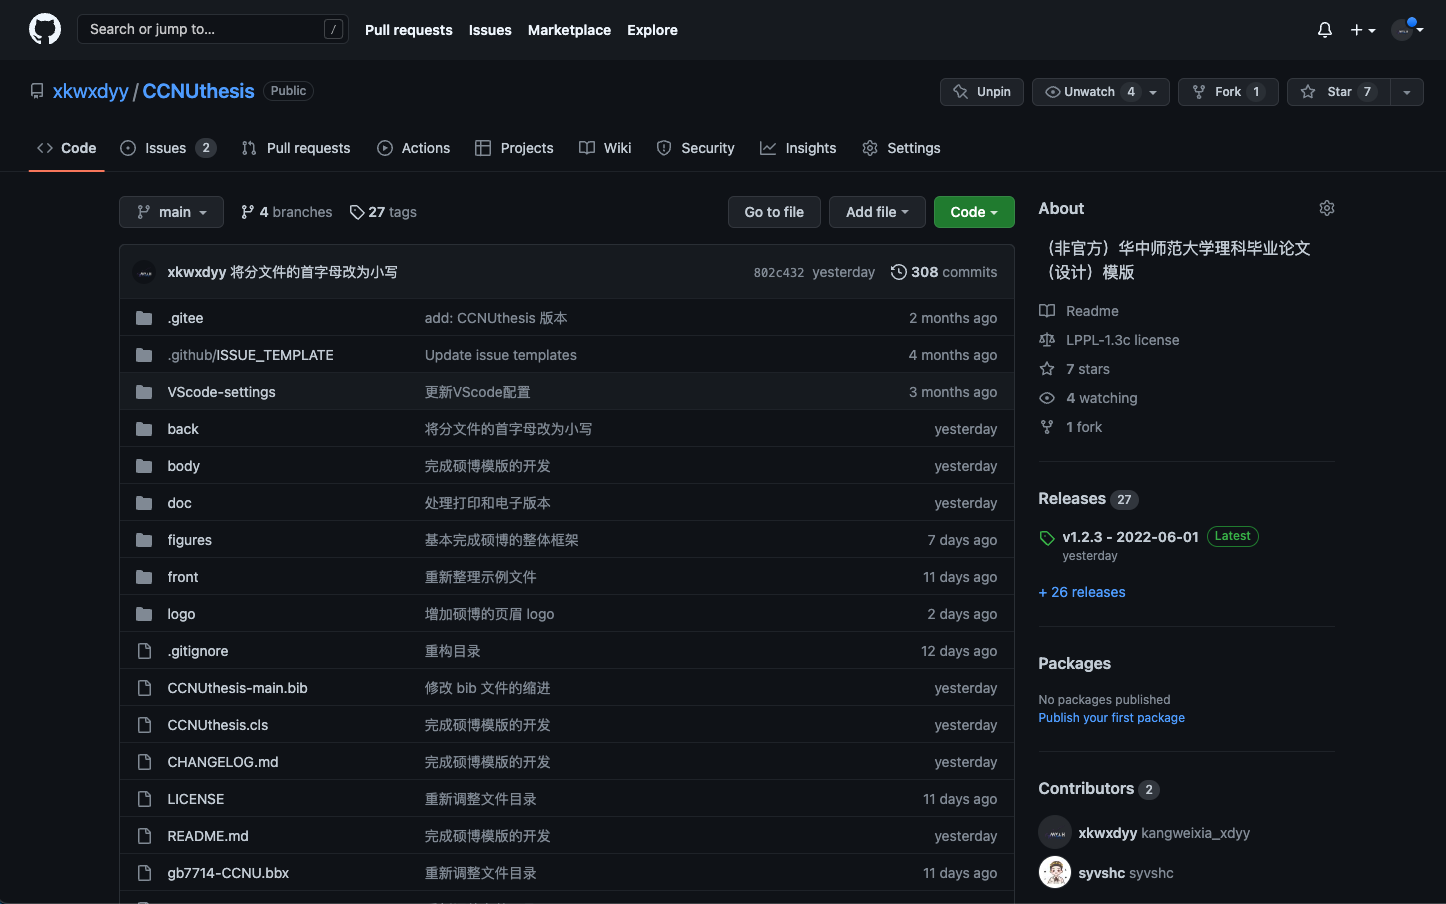
\includegraphics[width = \textwidth]{github项目主页.png}
  \caption{github 项目主页}
  \label{figure:github项目主页}
\end{figure}

\begin{figure}[htbp]
  \centering
  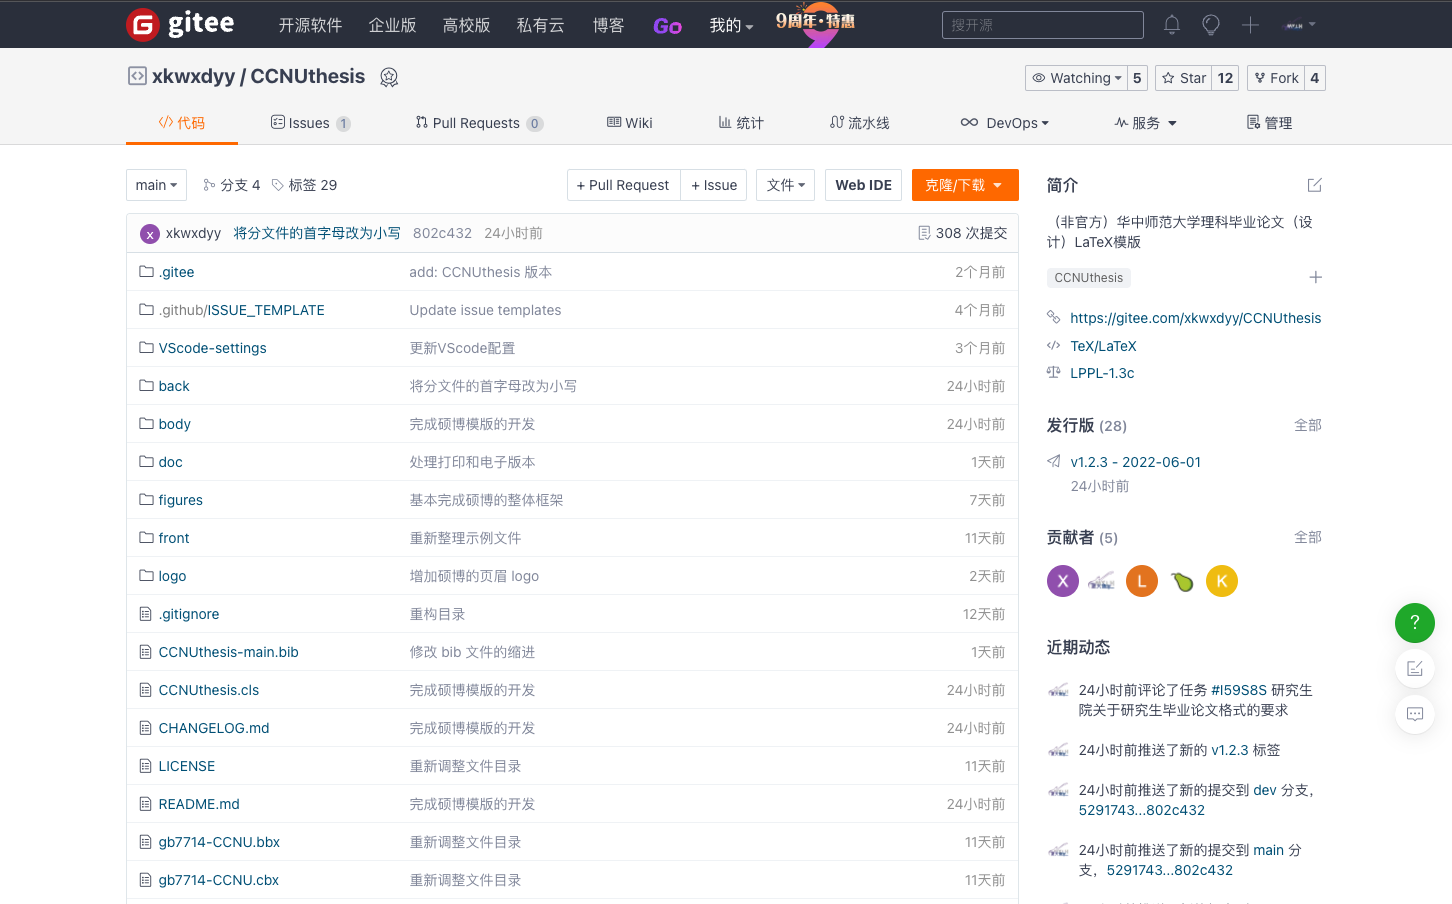
\includegraphics[width = \textwidth]{gitee项目主页.png}
  \caption{gitee 项目主页}
  \label{figure:gitee项目主页}
\end{figure}


\begin{figure}[htbp]
  \centering
  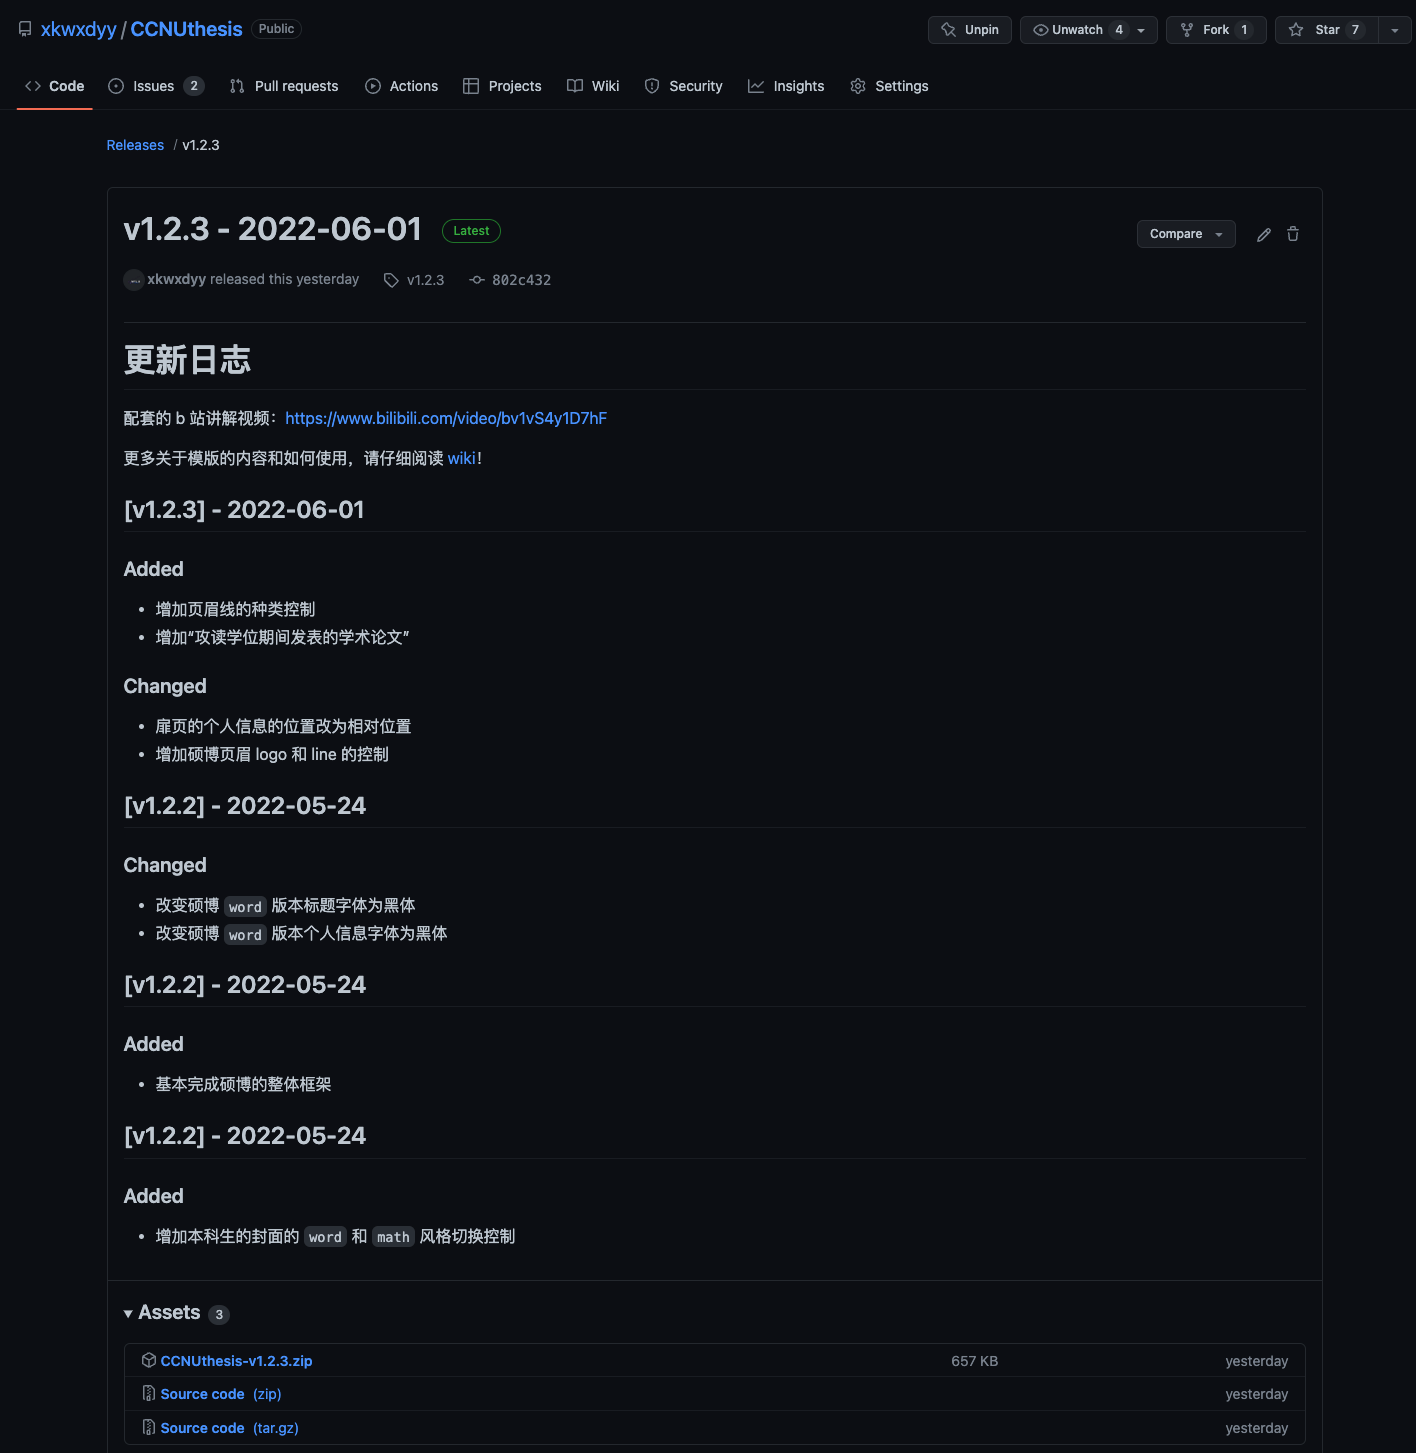
\includegraphics[width = \textwidth]{github发行版.png}
  \caption{github 发行版}
  \label{figure:github发行版}
\end{figure}

\begin{figure}[htbp]
  \centering
  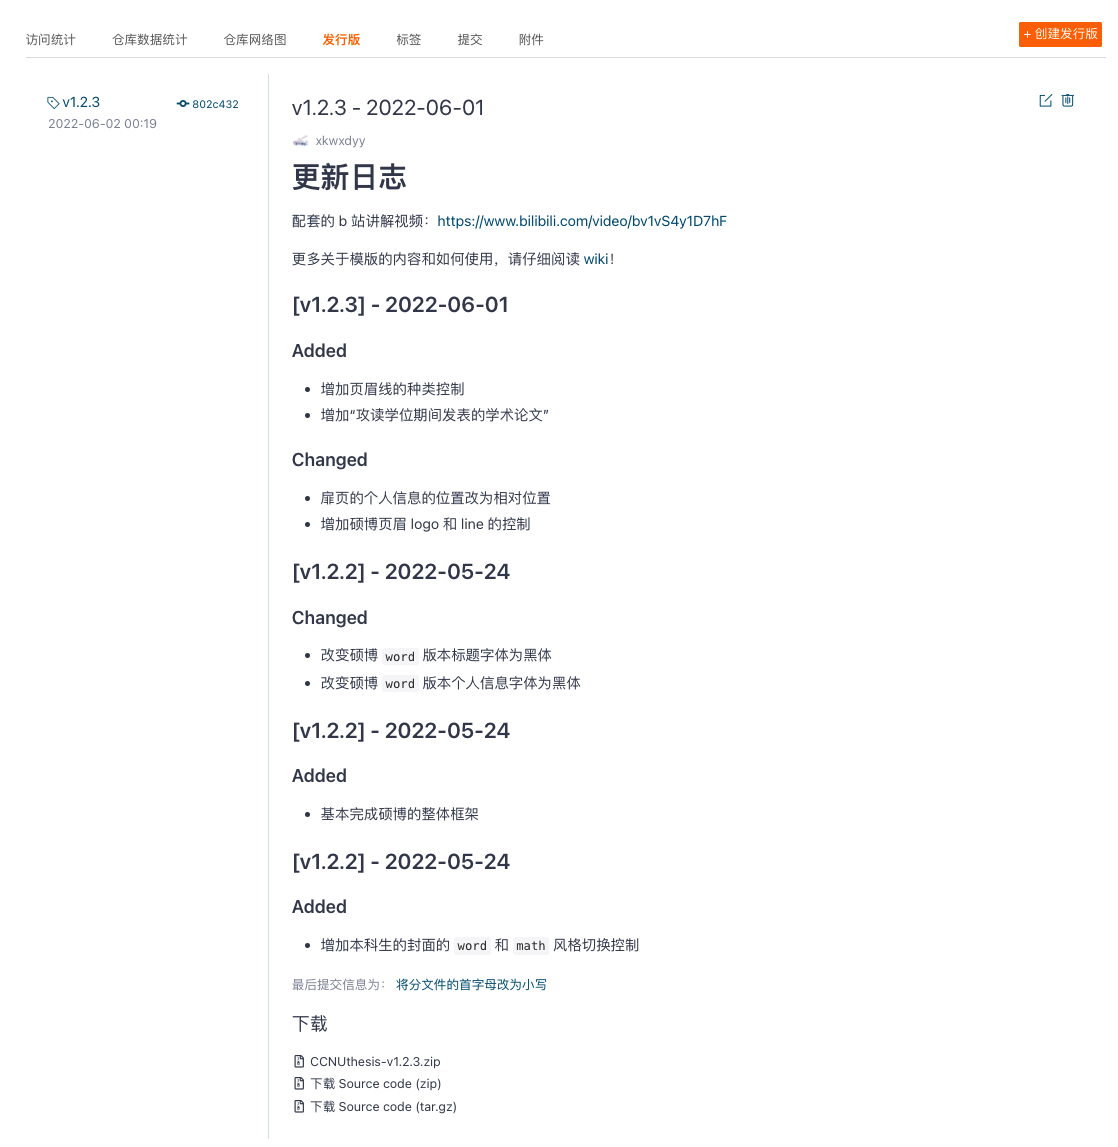
\includegraphics[width = \textwidth]{gitee发行版.png}
  \caption{gitee 发行版}
  \label{figure:gitee发行版}
\end{figure}

% \subsubsection{标准安装}

% 如果没有特殊理由,始终建议您使用宏包管理器安装 \cls{CCNUthesis}。
% 例如在 \TeXLive{} 中,执行(可能需要管理员权限)
% \begin{shellexample}[morekeywords={tlmgr,install}]
%   tlmgr install CCNUthesis
% \end{shellexample}
% 即可完成安装。

% 在 \TeXLive{} 和 \MiKTeX{} 中,您还可以通过图形界面进行安装,
% 此处不再赘述。

% \subsubsection{手动安装}

% 如果您需要从 CTAN 上自行下载并手动安装,较好的方法是使用 TDS
% 安装包:
% \begin{itemize}
%   \item 从 CTAN 上下载 \cls{CCNUthesis} 的
%     \href{http://mirror.ctan.org/install/macros/latex/contrib/CCNUthesis.tds.zip}{TDS 安装包};
%   \item 按目录结构将 \file{CCNUthesis.tds.zip} 中的文件复制到 \TeX{}
%     发行版的本地 TDS 根目录;
%   \item 执行 \bashcmd{mktexlsr} 刷新文件名数据库以完成安装。
% \end{itemize}
% %
% 您也可以从源代码直接生成模板(不推荐):
% \begin{itemize}
%   \item 打开 \href{https://github.com/stone-zeng/CCNUthesis}{项目主页},
%     点击“Code”按钮,并选择“Download ZIP”,下载 \file{CCNUthesis-main.zip};
%     如果您的电脑中安装有 git 程序,也可通过以下命令直接克隆代码仓库:
%     \begin{shellexample}[gobble=6,alsoletter={.},morekeywords={git,clone}]
%       git clone https://github.com/stone-zeng/CCNUthesis.git
%     \end{shellexample}
%   \item 解压并进入到 \file{source} 文件夹,执行以下命令以生成
%     模板的各组件:
%     \begin{shellexample}[gobble=6,morekeywords={xetex}]
%       xetex CCNUthesis.dtx
%     \end{shellexample}
%   \item 将生成的文档类(\file{.cls})、宏包(\file{.sty})以及
%     参数配置文件(\file{.def})复制到 \TeX{} 发行版本地 TDS 树
%     的 \path{texmf-local/tex/latex/CCNUthesis/} 目录下,并执行
%     \bashcmd{mktexlsr} 刷新文件名数据库,方可完成安装。
%   \item 使用 \cls{CCNUthesis} 撰写论文时,您还需要从代码仓库下的
%     \file{testfiles/support} 目录中复制 \file{fudan-name.pdf}
%     文件至工作目录,以确保封面中的校名图片可以正确显示。
% \end{itemize}

% \subsubsection{扁平化安装}

% 如果您不希望安装本模板,但需要立刻使用,也可以使用模板提供的安装脚本。
% 从 GitHub 上获取代码仓库后,执行 \file{install-win.bat}(Windows 系统)
% 或 \file{install-linux.sh}(Linux 系统),所有需要的文件便会在
% \file{thesis} 文件夹中生成。


\subsection{模板组成}

本模板主要包含核心文档类、参考文献格式文件以及用户文档等几个部分,
其具体组成见表~\ref{tab:ccnuthesis-main-components},模版子目录中的文件组成见表~\ref{tab:ccnuthesis-sub-components}。

\begin{table}[htbp]
  \caption{\cls{CCNUthesis} 的主要组成部分}
  \label{tab:ccnuthesis-main-components}
  \centering
  \small
  \begin{tblr}{
    hline{1, 2, Z} = {1pt},
    width = \textwidth,
    colspec = {X[2,l]X[5,l]},
    rows = {m}
  }
    \textbf{文件} & \textbf{功能说明} \\
    \file{CCNUthesis.pdf}         & 用户手册(本文档) \\
    \file{lguide-ch1.pdf}         & \TeXLive 安装指导 \\
    \file{main.tex}               & 模板的主文件,可据此为基础完成论文撰写 \\
    \file{ccnu-setup.tex}         & 用户的个人信息和论文相关参数设置的配置文件\\
    \file{CCNUthesis.cls}         & 模板文档类 \\
    \file{CCNUthesis-main.bib}    & 参考文献数据库文件,里面的条目均为示例,可删除后输入用户自己的参考文献条目并在正文中进行引用 \\
    {\file{gb7714-CCNU.bbx} \\ \file{gb7714-CCNUay.bbx}} & 参考文献的条目格式文件 \\
    \file{gb7714-CCNU.cbx}        & 参考文献的引用格式文件 \\
    \file{latexmkrc}              & \pkg{latexmk} 编译命令的配置文件 \\
    \file{README.md}              & 简要自述 \\
    \file{CHANGELOG.md}           & 模板更新日志 \\
    \file{LICENSE}                & 模版发布许可证
  \end{tblr}
\end{table}

\begin{table}[htbp]
  \caption{\cls{CCNUthesis} 各目录的组成部分}
  \label{tab:ccnuthesis-sub-components}
  \centering
  \small
  \begin{tblr}{
    hline{4,5,8,11,13} = {solid},
    hline{1, 2, Z} = {1pt},
    width = \textwidth,
    colspec = {X[1,l]X[3,l]X[3,l]},
    rows = {m},
    cell{2}{1} = {r=2}{m},
    cell{5}{1} = {r=3}{m},
    cell{8}{1} = {r=3}{m},
    cell{11}{1} = {r=2}{m},
  }
    \textbf{子目录} & \textbf{子目录中的文件} & \textbf{功能说明} \\
    front & \file{abstract.tex}            & 中英文摘要 \\
    front & \file{notation.tex}            & 符号表 \\
    body  & \file{chapter<number>.tex}     & 正文的分文件 \\
    back  & \file{acknowledgements.tex}    & 致谢 \\
    back  & \file{appendix.tex}            & 附录 \\
    back  & \file{publications.tex}        & 攻读学位期间取得的研究成果(博士)\\
    logo  & \file{ccnulogo.png}            & “华中师范大学”字样 logo \\
    logo  & \file{masterlogo.png}          & 硕士学位论文页眉 logo \\
    logo  & \file{doctorlogo.png}          & 博士学位论文页眉 logo \\
    copyright  & \file{Originality_Copyright.pdf}  & 本科学位论文原创性声明和使用授权说明 \\
    copyright  & \file{Originality_Copyright_master_doctor.pdf}  & 硕博学位论文原创性声明和使用授权说明\\
    figures & & 用户放置图片的目录\\
  \end{tblr}
\end{table}
% 使用介绍
% !TeX root = ../CCNUthesis-doc.tex

\section{使用说明}

\subsection{基本用法}

以下是一份简单的 \TeX{} 文档,它演示了 \cls{CCNUthesis} 的最基本用法:

\begin{latexexample}[deletetexcs={\documentclass},
    moretexcs={\chapter},morekeywords={\documentclass},
    emph={[2]document}]
  % main.tex
  \documentclass{CCNUthesis}
  \begin{document}
    \chapter{欢迎}
    \section{Welcome to CCNUthesis!}
    你好,\LaTeX{}!
  \end{document}
\end{latexexample}


按照~\ref{subsec:编译方式} 小节中的方式编译该文档,您应当得到一篇 3 页的文章。

% 英文模板可以用类似的方式使用:

% \begin{latexexample}[deletetexcs={\documentclass},
%     moretexcs={\chapter},morekeywords={\documentclass},
%     emph={[2]document}]
%   % thesis-en.tex
%   \documentclass{CCNUthesis-en}
%   \begin{document}
%     \chapter{Welcome}
%     \section{Welcome to CCNUthesis!}
%     Hello, \LaTeX{}!
%   \end{document}
% \end{latexexample}

% 英文模板只对正文部分进行了改动,封面、指导小组成员以及声明页仍将
% 显示为中文。

\subsection{编译方式} \label{subsec:编译方式}

本模板不支持 \pdfTeX{} 引擎,仅支持使用 \XeLaTeX{} 。为了生成正确的目录、脚注以及交叉引用,您至少需要连续编译两次。

以下代码中,假设您的 \TeX{} 源文件名为 \file{main.tex}。请在命令行中执行
\begin{shellexample}[morekeywords={xelatex}]
  xelatex main
\end{shellexample}

如果您想要编译参考文献,在 \file{CCNUthesis-main.bib} 中输入正确的条目信息并在正文中正确引用之后(引用方式见~\ref{para:参考文献引用}),请使用“\pkg{biber}”编译链,即在命令行中一次执行下面四条命令:
\begin{shellexample}[morekeywords={biber}]
  xelatex main
  biber main
  xelatex main
  xelatex main
\end{shellexample}
或使用 \pkg{latexmk}:
\begin{shellexample}[morekeywords={latexmk}]
  latexmk main
\end{shellexample}


\subsection{模板选项}

所谓“模板选项”,指需要在引入文档类的时候指定的选项:
\begin{latexexample}[deletetexcs={\documentclass},
    morekeywords={\documentclass}]
  \documentclass(*\oarg{模板选项}*){CCNUthesis}
\end{latexexample}

有些模板选项为布尔型,它们只能在 \opt{true} 和 \opt{false}
中取值。对于这些选项,\kvopt{\meta{选项}}{true} 中的“|= true|”
可以省略。

下面用形如“【本|硕|博】”表示该命令或环境的适用范围,比如“【硕|博】”表示输入之后仅对硕博模版起作用,对本科模版不起作用(作用范围的设置往往来源于格式规范的要求等),其余“【本】”等同理解释。


\begin{function}{type}
  \begin{ccnusyntax}[emph={[1]type}]
    type = (*<doctor|master|(bachelor)>*)
  \end{ccnusyntax}
  选择论文类型。三种选项分别代表博士学位论文、硕士学位论文和本科
  毕业论文。
\end{function}

\begin{function}[updated = 2022-06-20]{version}
  \begin{ccnusyntax}[emph={[1]version}]
    version = (*<(electronic)|print-master-oneside|print-master-twoside|print-doctor-twoside>*)
  \end{ccnusyntax}
  文档版本。
\end{function}

\begin{itemize}
  \item electronic:电子版,无空白页(本科选择这个即可,单双打印皆可,答辩时可以双面打印,纸质版终稿教务处要求单面打印)
  \item print-master-oneside:打印版,硕士,无空白页,单面打印
  \item print-master-twoside:打印版,硕士,有空白页,双面打印
  \item print-doctor-twoside:打印版,博士,有空白页,双面打印
\end{itemize}

注意:对于硕博的模版,\parencite{研究生院研究生学位论文规范} 中提到的“封面、原创性声明和使用授权书采用单面印刷,中英文扉页、摘要及后续内容采用双面印刷(硕士学位论文可以单面印刷)。” 实现方式即为在所需要单面印刷的后面加一页空白页,然后全部双面打印即可,这个就是上面键值的设计想法,用户不需要自己手动加空白页,只需要选择自己对应所需版本就会对应自动判断是否添加空白页。


% \begin{function}{oneside,twoside}
%   指明论文的单双面模式,默认为 \opt{twoside}。该选项会影响每章
%   的开始位置,还会影响页眉样式。
% \end{function}

% 在双面模式(\opt{twoside})下,按照通常的排版惯例,每章应只从
% 奇数页(在右)开始;而在单页模式(\opt{oneside})下,则可以从
% 任意页面开始。本模板中,目录、摘要、符号表等均视作章,也按相同
% 方式排版。

% 双面模式下,正文部分偶数页(在左)的左页眉显示章标题,奇数页
% (在右)的右页眉显示节标题;前置部分的页眉按同样格式显示,但文字
% 均为对应标题(如“目录”、“摘要”等)。
% 而在单面模式下,正文部分则页面不分奇偶,均同时显示左、右页眉,
% 文字分别为章标题和节标题;前置部分只有中间页眉,显示对应标题。

\begin{function}{draft}
  \begin{ccnusyntax}[emph={[1]draft}]
    draft = (*<\TFF>*)
  \end{ccnusyntax}
  【本|硕|博】选择是否开启草稿模式,默认关闭。
\end{function}

草稿模式为全局选项,会影响到很多宏包的工作方式。
开启之后,主要的变化有:
\begin{itemize}
  \item 把行溢出的盒子显示为黑色方块;
  \item 不实际插入图片,只输出一个占位方框;
  \item 关闭超链接渲染,也不再生成 PDF 书签;
  \item 显示页面边框。
\end{itemize}

% \begin{function}[added=2018-01-31]{config}
%   \begin{ccnusyntax}[emph={[1]config}]
%     config = (*\marg{文件}*)
%   \end{ccnusyntax}
%   用户配置文件的文件名。默认为空,即不载入用户配置文件。
% \end{function}


\subsection{参数设置}

\begin{function}{\ccnusetup}
  \begin{ccnusyntax}[morekeywords={\ccnusetup}]
    \ccnusetup(*\marg{键值列表}*)
  \end{ccnusyntax}
  【本|硕|博】本模板提供了一系列选项,可由您自行配置。载入文档类之后,以下
  所有选项均可通过统一的命令 \cs{ccnusetup} 来设置。
\end{function}

\cs{ccnusetup} 的参数是一组由(英文)逗号隔开的选项列表,列表中的
选项通常是 \kvopt{\meta{key}}{\meta{value}} 的形式。部分选项的
\meta{value} 可以省略。对于同一项,后面的设置将会覆盖前面的设置。
在下文的说明中,将用\textbf{粗体}表示默认值。

\cs{ccnusetup} 采用 \LaTeX3 风格的键值设置,支持不同类型以及多种
层次的选项设定。键值列表中,“|=|”左右的空格不影响设置;但需注意,
参数列表中\emph{不可以出现空行}。

与模板选项相同,布尔型的参数可以省略 \kvopt{\meta{选项}}{true}
中的“\kvopt{}{true}”。

另有一些选项包含子选项,如 \opt{style} 和 \opt{info} 等。它们可以
按如下两种等价方式来设定:

\begin{latexexample}[morekeywords={\ccnusetup},
    emph={[1]style,cjk-font,info,title,title*,author,author*,department}]
  \ccnusetup{
    style = {cjk-font = mac},
    info  = {
      title      = {论动体的电动力学},
      title*     = {On the Electrodynamics of Moving Bodies},
      author     = {阿尔伯特·爱因斯坦},
      author*    = {Albert Einstein},
      department = {物理学系}
    }
  }
\end{latexexample}

或者

\begin{latexexample}[morekeywords={\ccnusetup},
    emph={[1]style,cjk-font,info,title,title*,author,author*,department}]
  \ccnusetup{
    style/cjk-font  = mac,
    info/title      = {论动体的电动力学},
    info/title*     = {On the Electrodynamics of Moving Bodies},
    info/author     = {阿尔伯特·爱因斯坦},
    info/author*    = {Albert Einstein},
    info/department = {物理学系}
  }
\end{latexexample}


注意 “|/|” 的前后均不可以出现空白字符。


\subsubsection{论文格式} \label{subsubsec:论文格式}

\begin{function}{style}
  \begin{ccnusyntax}[emph={[1]style}]
    style = (*\marg{键值列表}*)
    style/(*\meta{key}*) = (*\meta{value}*)
  \end{ccnusyntax}
  【本|硕|博】该选项包含许多子项目,用于设置论文格式。具体内容见下。
\end{function}


\begin{function}{style/font}
  \begin{ccnusyntax}[emph={[1]font}]
    font = (*<newtx|(times)|stixtwo|xits|tg|none>*)
  \end{ccnusyntax}
  【本|硕|博】设置西文字体(包括数学字体)。具体配置见表~\ref{tab:font}。
\end{function}

% \begin{table}[ht]
% \centering
% \begin{threeparttable}
%   \caption{西文字体配置}
%   \label{tab:font}
%   \small
%   \begin{tabular}{ccccc}
%     \toprule
%       & \textbf{正文字体} & \textbf{无衬线字体} & \textbf{等宽字体} & \textbf{数学字体} \\
%     \midrule
%       |garamond|        & EB Garamond         & Libertinus Sans & LM Mono\tnote{a} & Garamond Math   \\
%       |libertinus|      & Libertinus Serif    & Libertinus Sans & LM Mono          & Libertinus Math \\
%       |lm|              & LM Roman            & LM Sans         & LM Mono          & LM Math         \\
%       |palatino|        & TG Pagella\tnote{b} & Libertinus Sans & LM Mono          & TG Pagella Math \\
%       |times|           & XITS                & TG Heros        & TG Cursor        & XITS Math       \\
%       |times*|\tnote{c} & Times New Roman     & Arial           & Courier New      & XITS Math       \\
%     \bottomrule
%   \end{tabular}
%   \begin{tablenotes}
%     \item[a] “LM”是 Latin Modern 的缩写。
%     \item[b] “TG”是 TeX Gyre 的缩写。
%     \item[c] 本行中,Times New Roman、Arial 和 Courier New 是商业字体,
%       不包含在 \TeXLive{} 发行版中,但在 Windows 和 macOS 系统上均默认安装。
%   \end{tablenotes}
% \end{threeparttable}
% \end{table}
\begin{table}[htbp]
  \centering
  \begin{threeparttable}
    \caption{西文字体配置}
    \label{tab:font}
    \small
    \begin{tabular}{ccccc}
      \toprule
        & \textbf{正文字体} & \textbf{无衬线字体} & \textbf{等宽字体} & \textbf{数学字体} \\
      \midrule
      |stixtwo| & STIX Two Text   & TG Heros\tnote{a} & TG Cursor   & STIX Two Math \\
      |xits |   & XITS            & TG Heros & TG Cursor   & XITS Math \\
      |times|\tnote{b}   & Times New Roman & Arial    & Courier New & newtxmath \\
      |newtx|   & TG Termes   & TG Heros & TG Cursor   & newtxmath \\
      |tg|      & TG Termes       & TG Heros & TG Cursor   & TG Termes Math \\
      \bottomrule
    \end{tabular}
    \begin{tablenotes}
      % \item[a] “LM”是 Latin Modern 的缩写。
      \item[a] “TG”是 TeX Gyre 的缩写。
      \item[b] 本行中,Times New Roman、Arial 和 Courier New 是商业字体,
        不包含在 \TeXLive{} 发行版中,但在 Windows 和 macOS 系统上均默认安装。
    \end{tablenotes}
  \end{threeparttable}
  \end{table}


\begin{function}{style/cjk-font}
  \begin{ccnusyntax}[emph={[1]cjk-font}]
    cjk-font = (*<adobe|(fandol)|founder|mac|sinotype|sourcehan|windows|none>*)
  \end{ccnusyntax}
  【本|硕|博】设置中文字体。具体配置见表~\ref{tab:cjk-font}。
\end{function}

\begin{table}[htbp]
  \caption{中文字体配置}
  \label{tab:cjk-font}
  \centering
  \small
  \begin{tabular}{ccccc}
    \toprule
      & \textbf{正文字体(宋体)} & \textbf{无衬线字体(黑体)} & \textbf{等宽字体(仿宋)} & \textbf{楷体} \\
    \midrule
      |adobe|     & Adobe 宋体      & Adobe  黑体     & Adobe  仿宋  & Adobe 楷体      \\
      |fandol|    & Fandol 宋体     & Fandol 黑体     & Fandol 仿宋  & Fandol 楷体     \\
      |founder|   & 方正书宋        & 方正黑体        & 方正仿宋     & 方正楷体        \\
      |mac|       & (华文)宋体-简 & (华文)黑体-简 & 华文仿宋     & (华文)楷体-简 \\
      |sinotype|  & 华文宋体        & 华文黑体        & 华文仿宋     & 华文楷体        \\
      |sourcehan| & 思源宋体        & 思源黑体        & ---          & ---             \\
      |windows|   & (中易)宋体    & (中易)黑体    & (中易)仿宋 & (中易)楷体    \\
    \bottomrule
  \end{tabular}
\end{table}

启用 \kvopt{font}{none} 或 \kvopt{cjk-font}{none} 之后,模板将关闭
默认西文 / 中文字体设置。此时,您需要自行使用 \cs{setmainfont}、
\cs{setCJKmainfont}、\cs{setmathfont} 等命令来配置字体。


% \begin{function}{style/font-size}
%   \begin{ccnusyntax}[emph={[1]font-size}]
%     font-size = (*<(-4)|5>*)
%   \end{ccnusyntax}

%   设置论文的基础字号。
% \end{function}


\begin{function}{style/fullwidth-stop}
  \begin{ccnusyntax}[emph={[1]fullwidth-stop}]
    fullwidth-stop = (*<catcode|mapping|(false)>*)
  \end{ccnusyntax}
  【本|硕|博】选择是否把全角实心句点\FSFW 作为默认的句号形状。
  这种句号一般用于科技类文章,以避免与下标“$_o$”或“$_0$”混淆。
\end{function}

选择 \kvopt{fullwidth-stop}{catcode} 或 \opt{mapping} 后,都会实现上述效果。
有所不同的是,在选择 \opt{catcode} 后,只有\emph{显式的}\FSID 会被替换
为\FSFW;但在选择 \opt{mapping} 后,\emph{所有的}\FSID 都会被替换。例如,
如果您用宏保存了一些含有\FSID 的文字,那么在选择 \opt{catcode} 时,其中
的\FSID 不会将被替换为\FSFW。

选项 \kvopt{fullwidth-stop}{mapping} 只在 \XeTeX{} 下有效。

如果您在选择 \kvopt{fullwidth-stop}{mapping} 后仍需要临时显示\FSID,
可以按如下方法操作:
\begin{latexexample}[moretexcs={\CJKfontspec},emph={[1]Mapping}]
  % 请使用 XeTeX 编译
  % 外侧的花括号表示分组
  这是一个句号{\CJKfontspec{(*\meta{字体名}*)}[Mapping=full-stop]。}
\end{latexexample}

\begin{function}{style/footnote-style}
% 这里奇怪的东西是用来控制对齐的。ccnusyntax 会吃掉开头的几个空格,因此这里用 X 来占位。
  \begin{ccnusyntax}[emph={[1]footnote-style}]
    footnote-style = (*<plain|\\
      XXXX\mbox{}~~~~~~~~~~~~~~~~~libertinus|libertinus*|libertinus-sans|\\
      XXXX\mbox{}~~~~~~~~~~~~~~~~~pifont|pifont*|pifont-sans|pifont-sans*|\\
      XXXX\mbox{}~~~~~~~~~~~~~~~~~xits|xits-sans|xits-sans*>*)
  \end{ccnusyntax}
  【本|硕|博】设置脚注编号样式。西文字体设置会影响其默认取值(见
  表~\ref{tab:footnote-font})。因此,要使得该选项生效,需将其
  放置在 \opt{font} 选项之后。带有 |sans| 的为相应的无衬线字体
  版本;带有 |*| 的为阴文样式(即黑底白字)。
\end{function}

\begin{table}[ht]
  \caption{西文字体与脚注编号样式默认值的对应关系}
  \label{tab:footnote-font}
  \centering
  \small
  \begin{tabular}{ccccc}
    \toprule
      \textbf{西文字体设置} &
        |libertinus| & |lm|     & |palatino| & |times| \\
    \midrule
      \textbf{脚注编号样式默认值} &
        |libertinus| & |pifont| & |pifont|   & |xits|  \\
    \bottomrule
  \end{tabular}
\end{table}

\begin{function}{style/caption-labelstyle}
  \begin{ccnusyntax}[emph={[1]caption-labelstyle}]
    caption-labelstyle = (*<arabic|(hyphen)|dot>*)
  \end{ccnusyntax}
  【本|硕|博】图表标题 label 计数样式。

  \begin{itemize}
    \item \opt{arabic}:图1,图2... 跨 chapter 连续编号,即若上一个 chapter 的图编号为 4,下一个 chapter 的第一个图编号为5
    \item \opt{hyphen}:图1-1,图1-2,图2-1...其中图 $x$-$y$,$x$ 表示 chapter 的值,$y$ 表示该 chapter 的计数器值(通俗理解就是此 chapter 的第 $y$ 张图或表),$y$ 在新的 chapter 会自动重新开始计数
    \item \opt{dot}:图1.1,图1.2,图2.1...其中图 $x$.$y$,$x,y$ 的含义同上
  \end{itemize}
\end{function}

\begin{function}{style/caption-labelseperator}
  \begin{ccnusyntax}[emph={[1]caption-labelseperator}]
    caption-labelseperator = (*<(colon)|space>*)
  \end{ccnusyntax}
  【本|硕|博】图表标题 label 和标题内容之间的分隔符

  \begin{itemize}
    \item \opt{colon}:表示 「:␣」,即一个西文冒号加一个空格
    \item \opt{space}:表示 「␣␣」,即两个空格
  \end{itemize}
\end{function}

\begin{function}[added = 2022-06-04]{style/chapter-breakstyle}
  \begin{ccnusyntax}[emph={[1]chapter-breakstyle}]
    caption-labelseperator = (*<(continuous)|newpage>*)
  \end{ccnusyntax}
  【本】控制 \tn{chapter} 是否新起一页。根据 \parencite{研究生院研究生学位论文规范},硕博模版的 \tn{chapter} 是新起一页的,故此键值设计仅对本科模版生效。

  \begin{itemize}
    \item \opt{continuous}:不新起一页,接着上一个 \tn{chapter} 连续排版
    \item \opt{newpage}:\tn{chapter} 会新起一页开始排版
  \end{itemize}
\end{function}

\begin{function}[added = 2022-06-20]{style/show-head}
  \begin{ccnusyntax}[emph={[1]show-head}]
    show-head = (*<\TTF>*)
  \end{ccnusyntax}
  【硕|博】是否显示页眉。统一控制页眉 logo 和页眉线的显示与否。
\end{function}


\begin{function}[updated = 2022-06-20]{style/show-headlogo}
  \begin{ccnusyntax}[emph={[1]show-headlogo}]
    show-headlogo = (*<\TFF>*)
  \end{ccnusyntax}
  【硕|博】是否显示页眉 logo。具体 logo 样式见图~\ref{figure:headlogo}。
\end{function}

\begin{figure}[htbp]
  \centering
  \begin{minipage}{0.45\textwidth}
    
\includegraphics[height = 2cm]{masterlogo.png}
  \end{minipage}
  \begin{minipage}{0.45\textwidth}
    
\includegraphics[height = 2cm]{doctorlogo.png}
  \end{minipage}
  \caption{headlogo}
  \label{figure:headlogo}
\end{figure}

\begin{function}{style/headline}
  \begin{ccnusyntax}[emph={[1]headline}]
    headline = (*<single|double|thin-thick|thick-thin|(none)>*)
  \end{ccnusyntax}
  【硕|博】页眉线的样式。

  \begin{itemize}
    \item \opt{single}:一条线
    \item \opt{double}:两条线,一样粗细
    \item \opt{thin-thick}:两条线,上细下粗(文武线)
    \item \opt{thick-thin}:两条线,上粗下细(武文线)
    \item \opt{none}:页眉没有线
  \end{itemize}
\end{function}

\begin{function}[added = 2022-6-19]{style/head-scope}
  \begin{ccnusyntax}[emph={[1]head-scope}]
    head-scope = (*<all|(main)>*)
  \end{ccnusyntax}
  【硕|博】页眉线的作用范围。

  \begin{itemize}
    \item \opt{all}:除了全文的第一页封面,其他页面均有页眉。
    \item \opt{main}:正文开始才有页眉。
  \end{itemize}
\end{function}

\begin{function}[added = 2022-06-18]{style/keywords-newline}
  \begin{ccnusyntax}[emph={[1]keywords-newline}]
    keywords-newline = (*\TTF*)(硕|博)
    keywords-newline = (*\TFF*)(本)
  \end{ccnusyntax}
  【本|硕|博】(中英统一控制)摘要和关键词之间是否空一行。

  \begin{itemize}
    \item \opt{true}:摘要和关键词之间空一行
    \item \opt{false}:摘要新起一段后为关键词
  \end{itemize}
\end{function}

\begin{function}[added = 2022-06-19]{style/listoffigures-show,style/listoftables-show}
  \begin{ccnusyntax}[emph={[1]listoffigures-show,listoftables-show}]
    listoffigures-show = (*\TTF*)(硕|博)
    listoftables-show = (*\TTF*)(硕|博)
    listoffigures-show = (*\TFF*)(本)
    listoftables-show = (*\TFF*)(本)
  \end{ccnusyntax}
  【本|硕|博】控制是否显示图表目录。若都显示则紧跟文章目录后,且图目录在表目录前。
\end{function}

\begin{function}[added = 2022-06-19]{style/listoffigures-name,style/listoftables-name}
  \begin{ccnusyntax}[emph={[1]listoffigures-name,listoftables-name}]
    listoffigures-name = (*<\marg{图目录的节标题}>*)
    listoftables-name = (*<\marg{表目录的节标题}>*)
  \end{ccnusyntax}
  【本|硕|博】图表目录的节标题。分别默认为 |插 \quad 图| 和 |表 \quad 格|
\end{function}


\begin{function}{style/hyperlink}
  \begin{ccnusyntax}[emph={[1]hyperlink}]
    hyperlink = (*<color|(none)>*)
  \end{ccnusyntax}
  【本|硕|博】设置超链接样式。\opt{color} 表示用彩色显示超链接;\opt{none} 表示没有特殊装饰,可用于生成最终的打印版文稿。
\end{function}

\begin{function}{style/hyperlink-color}
  \begin{ccnusyntax}[emph={[1]hyperlink-color}]
    hyperlink-color = (*<(default)|classic|material|graylevel|prl>*)
  \end{ccnusyntax}
  【本|硕|博】设置超链接颜色。该选项在 \kvopt{hyperlink}{none} 时无效。
  各选项所代表的颜色见表~\ref{tab:hyperlink-color}。
\end{function}


\begin{table}[ht]
\centering
\small

\newcommand\linkcolorexam[3]{%
  {\small 图~\textcolor[HTML]{#1}{1-2},
    (\textcolor[HTML]{#1}{3.4})~式} &
  {\small \textcolor[HTML]{#2}{\texttt{https://g.cn}}} &
  {\small 文献~[\textcolor[HTML]{#3}{1}],
    (\textcolor[HTML]{#3}{Knuth~1986})}}
\begin{threeparttable}
\caption{预定义的超链接颜色方案}
\label{tab:hyperlink-color}
\begin{tabular}{c*{3}{>{\hspace{0.2cm}}c<{\hspace{0.2cm}}}}
  \toprule
    \textbf{选项} & \textbf{链接} & \textbf{URL} & \textbf{引用} \\

  \midrule
    \opt{default}            & \linkcolorexam{990000}{0000B2}{007F00} \\
    \opt{classic}            & \linkcolorexam{FF0000}{0000FF}{00FF00} \\
    \opt{material}\tnote{a}  & \linkcolorexam{E91E63}{009688}{4CAF50} \\
    \opt{graylevel}\tnote{a} & \linkcolorexam{616161}{616161}{616161} \\
    \opt{prl}\tnote{b}       & \linkcolorexam{2D3092}{2D3092}{2D3092} \\
  \bottomrule
\end{tabular}
\begin{tablenotes}

  \item[a] 取自 Material 色彩方案
    (见 \url{https://material.io/guidelines/style/color.html})。
  \item[b] \textit{Physical Review Letter} 杂志配色。

\end{tablenotes}
\end{threeparttable}
\end{table}



% \begin{function}{style/bib-backend}
%   \begin{ccnusyntax}[emph={[1]bib-backend}]
%     bib-backend = (*<bibtex|biblatex>*)
%   \end{ccnusyntax}

%   选择参考文献的支持方式。选择 \opt{bibtex} 后,将使用 \BibTeX{}
%   处理文献,样式由 \pkg{natbib} 宏包负责;选择 \opt{biblatex} 后,
%   将使用 \biber{} 处理文献,样式则由 \pkg{biblatex} 宏包负责。
% \end{function}

\begin{function}{style/bib-style}
  \begin{ccnusyntax}[emph={[1]bib-style}]
    bib-style = (*<(ccnu-bachelor-numerical)|ccnu-bachelor-author-year|ccnu-master|ccnu-doctor|gb7714-2015>*)
  \end{ccnusyntax}
  【本|硕|博】设置参考文献样式。
  \begin{itemize}
    \item \opt{ccnu-bachelor-numerical}:参考 \parencite{本科生院毕业论文注释与参考文献著录格式} 定制的参考文献格式,顺序编码制
    \item \opt{ccnu-bachelor-author-year}:和 \opt{ccnu-bachelor-numerical} 格式相同,著者—出版年制
    \item \opt{ccnu-master}:国家标准 GB/T 7714--2015 的顺序编码制
    \item \opt{ccnu-doctor}:国家标准 GB/T 7714--2015 的顺序编码制
    \item \opt{gb7714-2015}:国家标准 GB/T 7714--2015 的顺序编码制
  \end{itemize}
  % \opt{author-year} 和 \opt{numerical} 分别对应国家标准 GB/T 7714--2015 \cite{gb-t-7714-2015} 中的著者—出版年制和顺序编码制。
  % 选择 \meta{其他样式} 时,如果 \kvopt{bib-backend}{bibtex},需保证相应的 \file{.bst} 格式文件能被调用;而如果\kvopt{bib-backend}{biblatex},则需保证相应的 \file{.bbx} 格式文件能被调用。
\end{function}

% \begin{function}{style/cite-style}
%   \begin{ccnusyntax}[emph={[1]cite-style}]
%     cite-style = (*\marg{引用样式}*)
%   \end{ccnusyntax}
%   选择引用格式。默认为空,即与参考文献样式(著者—出版年制或顺序
%   编码制)保持一致。如果手动填写,需保证相应的 \file{.cbx} 格式文件
%   能被调用。该选项在 \kvopt{bib-backend}{bibtex} 时无效。
% \end{function}

\begin{function}{style/bib-resource}
  \begin{ccnusyntax}[emph={[1]bib-resource}]
    bib-resource = (*\marg{文件}*)
  \end{ccnusyntax}
  【本|硕|博】参考文献数据源。可以是单个文件,也可以是用英文逗号隔开的一组文件。\emph{必须明确给出 \file{.bib} 后缀名}。默认为 \file{CCNUthesis-main.bib}。
\end{function}



\subsubsection{信息录入} \label{subsubsec:信息录入}

\begin{function}{info}
  \begin{ccnusyntax}[emph={[1]info}]
    info = (*\marg{键值列表}*)
    info/(*\meta{key}*) = (*\meta{value}*)
  \end{ccnusyntax}
  【本|硕|博】该选项包含许多子项目用于录入论文信息。具体内容见下。以下带“|*|”的项目表示对应的\emph{英文}字段或\emph{拼音}字段。
\end{function}

\begin{function}{info/cover-type}
  \begin{ccnusyntax}[emph={[1]cover-type}]
    cover-type  = (*<word|(math)>*)
  \end{ccnusyntax}
  【本|硕|博】封面类型。\opt{word} 表示几乎完全按照教务处给的 word 版本模版处理;\opt{math} 表示华中师范大学数学与统计学学院在 word 版本模版基础上进行部分细节调整。
\end{function}

\begin{function}[added = 2022-12-10]{info/title-line-type}
  \begin{ccnusyntax}[emph={[1]title-line-type}]
    title-line-type  = (*<variable|(constant)>*)
  \end{ccnusyntax}
  【本|硕|博】封面中文标题下划线类型。\opt{variable} 表示下划线只有文字出现的地方才有,也就是不会出现空白处有下划线的情况;\opt{constant} 表示下划线是恒定长度,可能会出现空白处处有下划线。
\end{function}

\begin{function}{info/title,info/title*}
  \begin{ccnusyntax}[emph={[1]title,title*}]
    title  = (*\marg{中文标题}*)
    title* = (*\marg{英文标题}*)
  \end{ccnusyntax}
  【本|硕|博】论文标题。默认会在约 21 个汉字(本科,硕博在 14 个汉字)字宽处自动断行,但为了语义的连贯以及排版的美观,如果您的标题长于一行,可以根据语义使用“|\\|”手动断行。如果您的标题中有副标题,使用“|\\|”手动断行并以“——”开头,如
\begin{latexexample}
  title = {
    如何使用 \LaTeX 编写论文模版 \\
    ——以华中师范大学为例
  }
\end{latexexample}
\end{function}

\begin{function}{info/author,info/author*}
  \begin{ccnusyntax}[emph={[1]author,author*}]
    author  = (*\marg{姓名}*)【本|硕|博】
    author* = (*\marg{姓名拼音)}*)【硕|博】
  \end{ccnusyntax}
  作者姓名。
\end{function}

\begin{function}{info/student-id}
  \begin{ccnusyntax}[emph={[1]student-id}]
    student-id  = (*\marg{学号}*)
  \end{ccnusyntax}
  【本】作者学号。
\end{function}

\begin{function}{info/level}
  \begin{ccnusyntax}[emph={[1]level}]
    level  = (*\marg{年级}*)
  \end{ccnusyntax}
  【本】年级。
\end{function}

\begin{function}{info/supervisor,info/supervisor*-name,info/supervisor*-academic-title}
  \begin{ccnusyntax}[emph={[1]supervisor,supervisor*-name,supervisor*-academic-title}]
    supervisor = (*\marg{姓名}*)【本|硕|博】
    supervisor*-name = (*\marg{姓名拼音}*)【硕|博】
    supervisor*-academic-title = (*\marg{职称英文}*)【硕|博】
  \end{ccnusyntax}
  导师姓名、职称。
\end{function}

\begin{function}{info/department,info/department*}
  \begin{ccnusyntax}[emph={[1]department,department*}]
    department = (*\marg{学院名称}*)【本|硕|博】
    department* = (*\marg{学院英文名称}*)【硕|博】
  \end{ccnusyntax}
  学院名称。
\end{function}

\begin{function}{info/major,info/major*}
  \begin{ccnusyntax}[emph={[1]major,major*}]
    major = (*\marg{专业名称}*)【本|硕|博】
    major* = (*\marg{专业英文名称}*)【硕|博】
  \end{ccnusyntax}
  专业名称。
\end{function}

\begin{function}{info/research-area,info/research-area*}
  \begin{ccnusyntax}[emph={[1]research-area,research-area*}]
    research-area = (*\marg{研究方向名称}*)【硕|博】
    research-area* = (*\marg{研究方向英文名称}*)【博】
  \end{ccnusyntax}
  作者研究方向。
\end{function}

\begin{function}{info/degree-type,info/degree-type*}
  \begin{ccnusyntax}[emph={[1]degree-type,degree-type*}]
    degree-type = (*\marg{申请学位学生类别}*)【硕|博】
    degree-type* = (*\marg{英文申请学位学生类别缩写}*)【硕】
  \end{ccnusyntax}
  申请学位学生类别。如
  \begin{itemize}
    \item 教育硕士|应用统计硕士|全日制硕士|同等学力人员|高校教师在职攻读硕士学位人员|专业学位人员
    \item 博士
  \end{itemize}
  英文缩写比如:M.S.
\end{function}


\begin{function}{info/keywords,info/keywords*}
  \begin{ccnusyntax}[emph={[1]keywords,keywords*}]
    keywords  = (*\marg{中文关键字}*)
    keywords* = (*\marg{英文关键字}*)
  \end{ccnusyntax}
  【本|硕|博】关键字列表。各关键字之间需使用 \emph{英文逗号} 隔开。
\end{function}


\begin{function}{info/year,info/month}
  \begin{ccnusyntax}[emph={[1]year,month}]
    year = (*\marg{年}*)
    month = (*\marg{月份}*)
  \end{ccnusyntax}
  【本|硕|博】论文完成的年月。默认值为文档编译时的年和月。
\end{function}



\subsection{正文编写}

\begin{quotation}
  喬孟符(吉)博學多能,以樂府稱。嘗云:「作樂府亦有法,
  曰\CJKunderdot{鳳頭、豬肚、豹尾}六字是也。」大概起要美麗,中要浩蕩,
  結要響亮。尤貴在首尾貫穿,意思清新。苟能若是,斯可以言樂府矣。
\end{quotation}
\hfill ——陶宗儀《南村輟耕錄·作今樂府法》


\subsubsection{凤头}

\begin{function}{\frontmatter}
  【本|硕|博】声明前置部分开始。
\end{function}

在本模板中,前置部分包含目录、中英文摘要以及符号表等。硕博模版的前置部分的页码采用小写罗马字母,并且与正文分开计数;本科模版采用阿拉伯数字,并与正文连续计数。本硕博模版目录均无页码。

目录会自动生成,无需用户手动控制。

\begin{function}{abstract}
  \begin{ccnusyntax}[emph={[2]abstract}]
    % abstract.tex
    \begin{abstract}
      (*\meta{中文摘要}*)
    \end{abstract}
  \end{ccnusyntax}
  【本|硕|博】中文摘要。
\end{function}
\begin{function}{abstract*}
  \begin{ccnusyntax}[emph={[2]abstract*}]
    % abstract.tex
    \begin{abstract*}
      (*\meta{英文摘要}*)
    \end{abstract*}
  \end{ccnusyntax}
  【本|硕|博】英文摘要。
\end{function}


\begin{function}{notation}
  \begin{ccnusyntax}[emph={[2]notation}]
    \begin{notation}(*\oarg{列格式说明}*)
      (*\meta{符号 1}*)  &  (*\meta{说明}*)  \\
      (*\meta{符号 2}*)  &  (*\meta{说明}*)  \\
      (*\phantom{\meta{符号 $n$}}*)  (*$\vdots$*)
      (*\meta{符号\ \kern-0.1em$n$}*)  &  (*\meta{说明}*)
    \end{notation}
  \end{ccnusyntax}
  【本|硕|博】符号表。基于 \pkg{tabularray} 宏包的 \env{longtblr} 环境,可选参数 \meta{列格式说明} 和 \env{longtblr} 环境的可选参数接口相同,并设置默认为
\begin{latexexample}
  width   = 0.3\textwidth,
  colspec = {X[1,c]X[1,c]}
\end{latexexample}
  如果效果不满意,请您命令行输入 \cmd{texdoc tabularray} 自行查阅 \pkg{tabularray} 宏包的用户手册了解更多使用参数和细节。
\end{function}

\subsubsection{猪肚}

\begin{function}{\mainmatter}
  【本|硕|博】声明主体部分开始。
\end{function}

主体部分是论文的核心,您可以分章节撰写。如有需求,也可以采用
多文件编译的方式。主体部分的页码采用阿拉伯数字。

\begin{function}{\footnote}
  \begin{ccnusyntax}[deletetexcs={\footnote},morekeywords={\footnote}]
    \footnote(*\marg{脚注文字}*)
  \end{ccnusyntax}
  【本|硕|博】插入脚注。脚注编号样式可利用 \opt{style/footnote-style} 选项控制,
  具体见 \ref{subsubsec:论文格式}~小节。

  需要注意的是,\parencite{本科生院毕业论文注释与参考文献著录格式} 中指出
  \begin{itemize}
    \item 文科术科的论文注释使用脚注
    \item 理工科的论文注释\textcolor{red}{\emph{不使用}}脚注
  \end{itemize}
\end{function}

\begin{function}{\caption}
  \begin{ccnusyntax}[deletetexcs={\caption},morekeywords={\caption}]
    \caption(*\marg{图表标题}*)
  \end{ccnusyntax}
  【本|硕|博】插入图表标题。
\end{function}

按照排版惯例,建议您将表格的标题放置在绘制表格的命令之前,
而将图片的标题放置在绘图或插图的命令之后。另需注意,
\tn{caption} 命令必须放置在浮动体环境(如 \env{table} 和
\env{figure})中。


\paragraph{参考文献引用}\label{para:参考文献引用}

\begin{function}{\parencite}
  \begin{ccnusyntax}[deletetexcs={\parencite},morekeywords={\parencite}]
    \parencite(*\marg{文献标签}*)
    \parencite(*\oarg{postnote}\marg{文献标签}*)
    \parencite(*\oarg{prenote}\oarg{postnote}\marg{文献标签}*)
  \end{ccnusyntax}
\end{function}

\begin{function}{\cite}
  \begin{ccnusyntax}[deletetexcs={\cite},morekeywords={\cite}]
    \cite(*\marg{文献标签}*)
    \cite(*\oarg{postnote}\marg{文献标签}*)
    \cite(*\oarg{prenote}\oarg{postnote}\marg{文献标签}*)
  \end{ccnusyntax}
\end{function}

【本|硕|博】插入所引用的文献。\meta{prenote} 和 \meta{posnote} 由名称可看出,一个是出现在前方,一个出现在后方。绝大部分情况只需用到可选参数 \meta{postnote},可用来标注引文的页码或引用的定理。

\tn{parencite} 是行内引用,\tn{cite} 是上标引用。通常情况下

\begin{itemize}
  \item 下面两种情况要用行内引用 \tn{parencite}:
    \begin{enumerate}
      \item 去掉这个引用句子结构不完整,比如“定理证明可参看[1]”
      \item 英文文献的引用
    \end{enumerate}
  \item 下面情况用上标引用 \tn{cite}:
    \begin{itemize}
      \item 去掉这个引用后句子结构仍然完整,比如“作者提到,CCNUthesis 是一个非常好的好模版$^{[1]}$。”
    \end{itemize}
\end{itemize}

如果您对上述的说法觉得不赞同或有所补充,欢迎提出!(可按~\ref{subsec:提issues} 节的链接到 \cls{CCNUthesis} 项目主页提 issues)

效果举例:

\begin{latexexample}
  % CCNUthesis-main.bib
  % @book{feynman2011,
  %   title     = {The Feynman lectures on physics, Vol. I: The new millennium edition: mainly mechanics, radiation, and heat},
  %   author    = {Feynman, Richard P and Leighton, Robert B and Sands, Matthew},
  %   volume    = {1},
  %   year      = {2011},
  %   publisher = {Basic books},
  %   pages     = {2-8},
  %   edition   = {7},
  %   url       = {https://arxiv.org/abs/2201.00067}
  % }

  % main.tex
  英文文献 \parencite{feynman2011}

  英文文献 \parencite[12]{feynman2011}

  英文文献 \parencite[Thm1]{feynman2011}

  英文文献 \parencite[12][Thm1]{feynman2011}

  英文文献 \cite{feynman2011}

  英文文献 \cite[12]{feynman2011}

  英文文献 \cite[Thm1]{feynman2011}

  英文文献 \cite[12][Thm1]{feynman2011}
\end{latexexample}

最终效果见图~\ref{figure:cite-parencite效果}(其中“4”仅为测试效果,具体取决于 \cmd{bib-style} 的样式及引用顺序等)。

\begin{figure}[htbp]
  \centering
  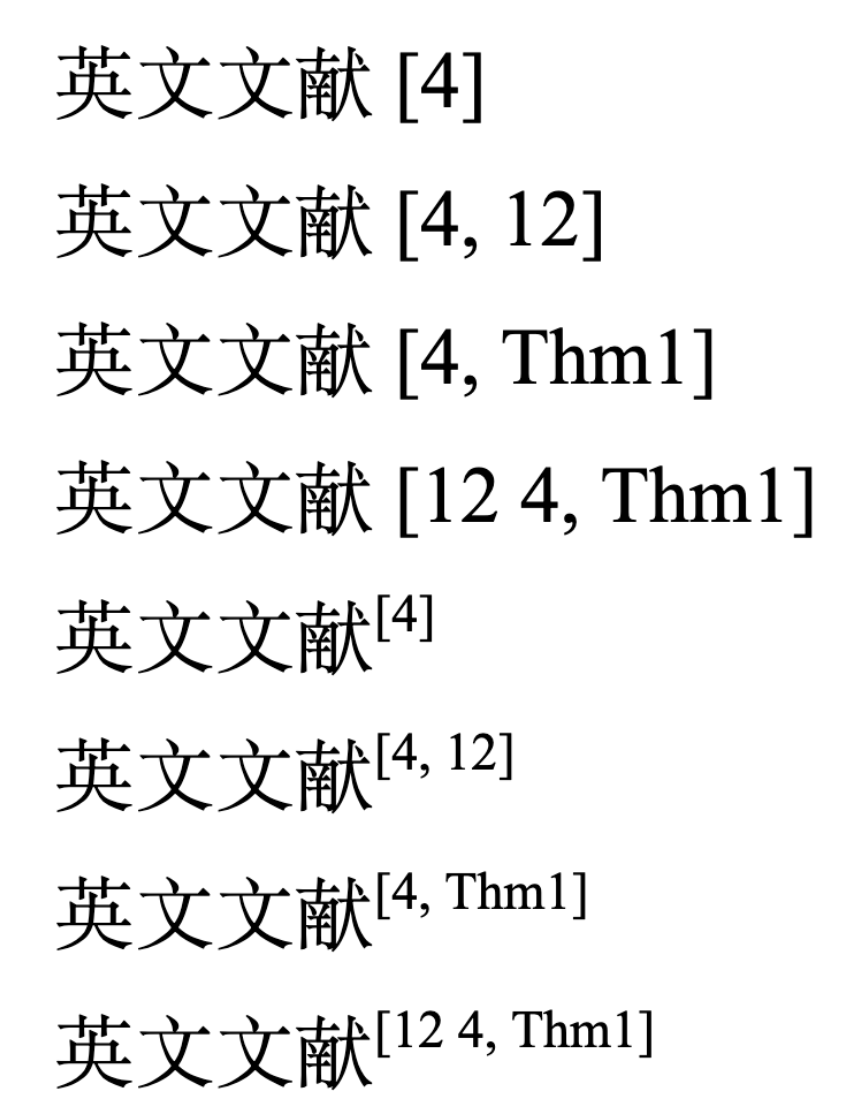
\includegraphics[width = 0.4\textwidth]{cite-parencite效果.png}
  \caption{\tn{cite} 和 \tn{parencite} 的效果}
  \label{figure:cite-parencite效果}
\end{figure}


\paragraph{定理类环境}


\begin{function}{axiom,counterexample,claim,corollary,conjecture,definition,example,lemma,property,proof,proposition,question,remark,theorem}
  \begin{ccnusyntax}[emph={[2]proof}]
    \begin{proof}(*\oarg{小标题}*)
      (*\meta{证明过程}*)
    \end{proof}
  \end{ccnusyntax}
  【本|硕|博】一系列预定义的数学环境。具体含义见表~\ref{tab:theorem}。
\end{function}

\begin{table}[ht]
  \caption{预定义的数学环境} \label{tab:theorem}
  \centering
  \small
  \begin{tblr}{
    width = \textwidth,
    columns = {c},
    hline{1,2,Z} = {solid}
  }
    \textbf{名称} &
      \env{axiom} & \env{counterexample} & \env{claim} & \env{corollary} & \env{conjecture} & \env{definition} & \env{example} \\
    \textbf{含义} &
      公理 & 反例 & 断言 & 推论 &
      猜想 & 定义 & 例 \\
  \end{tblr}

  \medskip

  \begin{tblr}{
    width = \textwidth,
    columns = {c},
    hline{1,2,Z} = {solid}
  }
    \textbf{名称} &
      \env{lemma} & \env{property} & \env{proof} & \env{proposition} & \env{question} & \env{remark} & \env{theorem} \\
    \textbf{含义} &
      引理 & 性质 & 证明 & 命题 &
      问题 & 注  & 定理 \\
  \end{tblr}
\end{table}

\begin{function}{\qedhere}
  【本|硕|博】证明环境(\env{proof})的最后会添加证毕符号“$\square$”。对于证明如果以公式结尾或其它某些情况时“$\square$”可能会出现在新的空白行的行尾,如果想要“$\square$”出现在“有内容的”行尾,可以在想要出现的地方使用 \tn{qedhere} 命令。
\end{function}

比如您可以在模版中测试下面代码查看效果:

\begin{latexexample}
  \begin{proof}
    \[
      x^2
    \]
  \end{proof}
  \begin{proof}
    \[
      x^2  \qedhere
    \]
  \end{proof}
\end{latexexample}


\begin{function}[added = 2022-06-04]{\ccnunewtheorem,\ccnunewtheorem*}
  \begin{ccnusyntax}[deletetexcs={\ccnunewtheorem,\ccnunewtheorem*},morekeywords={\ccnunewtheorem,\ccnunewtheorem*}]
    \ccnunewtheorem(*\oarg{计数器样式设置}\marg{环境中文名称}\marg{环境名}*)
    \ccnunewtheorem*(*\oarg{计数器样式设置}\marg{环境中文名称}\marg{环境名}*)
  \end{ccnusyntax}
  【本|硕|博】自定义定理类环境的命令。带星号的表示新定义的环境无计数器,类似于 \env{proof} 环境。
\end{function}

该命令的主要用法有下面四种:
\begin{latexexample}
  \ccnunewtheorem{测试}{test}
  \ccnunewtheorem*{测试试}{testt}
  \ccnunewtheorem[sibling = theorem]{测试试试}{testtt}
  \ccnunewtheorem[within = chapter]{测试试试试}{testttt}
\end{latexexample}

\begin{itemize}
  \item |\ccnunewtheorem{测试}{test}| 定义了一个 \env{test} 环境,label 名为 \env{测试}。环境自己用自己的计数器,并且跨 chapter 连续编号
  \item |\ccnunewtheorem*{测试试}{testt}| 定义了一个 \env{testt} 环境,label 名为 \env{测试试}。环境不编号。
  \item |\ccnunewtheorem[sibling = theorem]{测试试试}{testtt}| 定义了一个 \env{testtt} 环境,label 名为 \env{测试试试}。环境和 theorem 环境共用一个计数器。
  \item |\ccnunewtheorem[within = chapter]{测试试试试}{testttt}| 定义了一个 \env{testttt} 环境,label 名为 \env{测试试试试}。环境计数器的值和章节有关,形如 $x.y$,$x$ 表示章节的计数器的值,子计数器 $y$ 随新章节清零重新计数。
\end{itemize}

您可以看图~\ref{figure:ccnunewtheorem} 的效果来更好地理解四种用法的效果,

\begin{figure}[htbp]
  \centering
  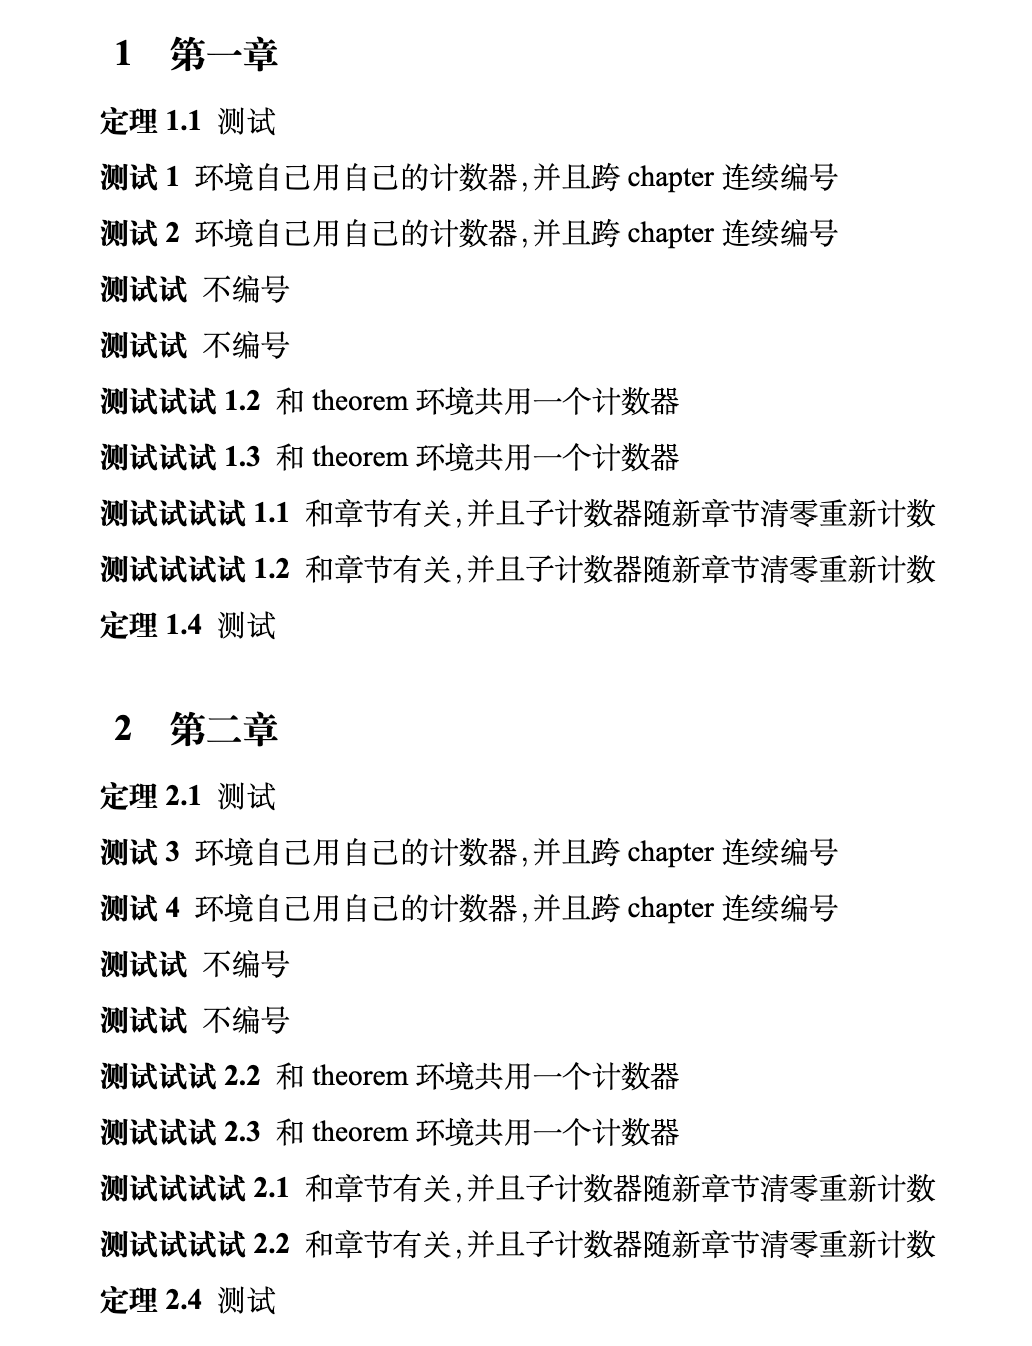
\includegraphics[width = 0.7\textwidth]{ccnunewtheorem.png}
  \caption{\tn{ccnunewtheorem} 示例}
  \label{figure:ccnunewtheorem}
\end{figure}



\subsubsection{豹尾}

\begin{function}{\backmatter}
  【本|硕|博】声明后置部分开始。
\end{function}

后置部分包含参考文献、声明页等。

\begin{function}{\printbibliography}
  \begin{ccnusyntax}[morekeywords={\printbibliography}]
    \printbibliography(*\oarg{选项}*)
  \end{ccnusyntax}
  【本|硕|博】打印参考文献列表。该命令由 \pkg{biblatex} 宏包直接提供,可用选项请参阅其文档。一般来说,用户不需要做任何改动。
\end{function}

\begin{function}{\acknowledgements}
  【本|硕|博】开启致谢章节。

\begin{latexexample}
  % acknowledgements.tex
  \acknowledgements
  
  <致谢内容>
\end{latexexample}
\end{function}

\begin{function}{signature}
  \begin{ccnusyntax}
    \begin{signature}
      <落款>
    \end{signature}
  \end{ccnusyntax}
  【本|硕|博】落款签名。整体右对齐,内部居中对齐。可用|\\|换行
\begin{latexexample}
  \begin{signature}
    夏康玮 \\
    2022年6月5日于珞珈山
  \end{signature}
\end{latexexample}
\end{function}


\begin{function}{\appendix}
  【本|硕|博】开启附录章节。
  
\begin{latexexample}
  % appendix.tex
  \appendix
  
  \chapter{<附录标题>}
  <附录内容>

  \chapter{<附录标题>}
  <附录内容>
\end{latexexample}

  附录和正文的章节层级相同,也是 \tn{chapter} 开始。需注意:\emph{硕博模版的附录在致谢前,本科模版的附录在致谢后。}

  根据 \parencite{研究生院研究生学位论文规范} 的要求“附录另起一页,“附录”两字居中,中间空两格,三号黑体加粗。如有多个附录,可用附录1、附录2区别并加以排序。” 模版已经做了自动化处理,即
  \begin{itemize}
    \item 如果 \file{appendix.tex} 中只有一个 \tn{chapter}\marg{内容} 的话,章节标题和目录中显示“附录 \meta{内容}”
    \item 如果 \file{appendix.tex} 中有两个及两个以上的 \tn{chapter}\marg{内容} 的话,章节标题和目录中显示“附录A \meta{内容}”、“附录B \meta{内容}”
  \end{itemize}
  但和一般的交叉引用不同,附录的此自动化处理,一般来说可能需要编译两次甚至三次,这个取决于用户在何时进行编译(比如编译之后又写了一个 \tn{chapter}\marg{内容} 的话,就需要三次编译才可以达到正确的章节标题和目录内容),但是三次(只要附录外的内容没问题,附录内没有报错)一定可以达到正确的编译效果。
\end{function}


\begin{function}{\publication}
  【博】开启“攻读学位期间取得的研究成果”章节。
\end{function}

\begin{function}{publications}
  \begin{ccnusyntax}[emph={[2]publications}]
    \begin{publications}
      \item (*\meta{研究成果1}*)
      \item (*\meta{研究成果2}*)
      ...
    \end{publications}
  \end{ccnusyntax}
  【博】研究成果列表环境。研究成果的格式等需要用户自行输入,无法像参考文献一样自动化,具体的字体字样等命令请自行查阅 \href{https://ctan.math.illinois.edu/info/lshort/chinese/lshort-zh-cn.pdf}{lshort-zh-cn}。
\end{function}

博士模版使用只需要取消 \file{main.tex} 中的
\begin{latexexample}
  % % !TeX root = ../main.tex
\publication


\begin{publications}
  \item test
  \item test
  \item test
  \item test
  \item test
  \item test
  \item test
  \item test
  \item test
  \item test
  \item test
  \item test
  \item test
  \item test
  \item test
  \item test
\end{publications}
\end{latexexample}
的代码注释,并且在 \file{publications.tex} 文件中输入相应内容然后编译即可。

\begin{function}{choices}
  \begin{ccnusyntax}[emph={[2]choices}]
    \begin{choices}(*\oarg{可选参数}*)
      \item (*\meta{选项1}*)
      \item (*\meta{选项2}*)
      ...
    \end{choices}
  \end{ccnusyntax}
  【本|硕|博】选项排版环境。对于有排版试卷、问卷等需求的用户,此环境能方便地帮您进行任意个选项的排版,并可以方便地调整选项 label 的样式。
\end{function}

用法和列表环境相同,使用 \tn{item} 分隔选项。label 的样式支持

\begin{itemize}
  \item arabic(阿拉伯数字)
  \item alph(小写英文)
  \item Alph(大写英文)
  \item roman(小写罗马数字)
  \item Roman(大写罗马数字)
  \item circlednumber(带圈数字)
\end{itemize}

如
\begin{latexexample}
  \begin{choices}[label = \arabic*)]
    \item 选项1
    \item 选项2
    \item 选项3
    \item 选项4
  \end{choices}
  
  \begin{choices}[label = (\alph*]
    \item 选项1
    \item 选项2
    \item 选项3
    \item 选项4
  \end{choices}
  
  \begin{choices}[label = \Alph*.]
    \item 选项1
    \item 选项2
    \item 选项3
    \item 选项4
  \end{choices}
  
  \begin{choices}[label = \roman*:]
    \item 选项1
    \item 选项2
    \item 选项3
    \item 选项4
  \end{choices}
  
  \begin{choices}[label = \Roman*-]
    \item 选项1
    \item 选项2
    \item 选项3
    \item 选项4
  \end{choices}
  
  \begin{choices}[label = \circlednumber*]
    \item 选项1
    \item 选项2
    \item 选项3
    \item 选项4
    \item 选项5
    \item 选项6
    \item 选项7
    \item 选项8
  \end{choices}
\end{latexexample}


还可以修改 \opt{columns} 键值来决定每行排多少个
\begin{latexexample}
  \begin{choices}[
    columns = 3,            % 手动控制每行多少个选项,否则自己根据宽度自动排版
    label   = (\arabic*)      % label 的样式,支持 arabic, alph, Alph, roman, Roman, circlednumber
  ]
    \item 选项1
    \item 选项2
    \item 选项3
    \item 选项4
    \item 选项5
    \item 选项6
  \end{choices}
\end{latexexample}

具体效果可见~\ref{figure:choices环境示例}。更多关于 \env{choices} 环境的精细调整可以查看 \url{https://gitee.com/zepinglee/exam-zh}。

\begin{figure}[htbp]
  \centering
  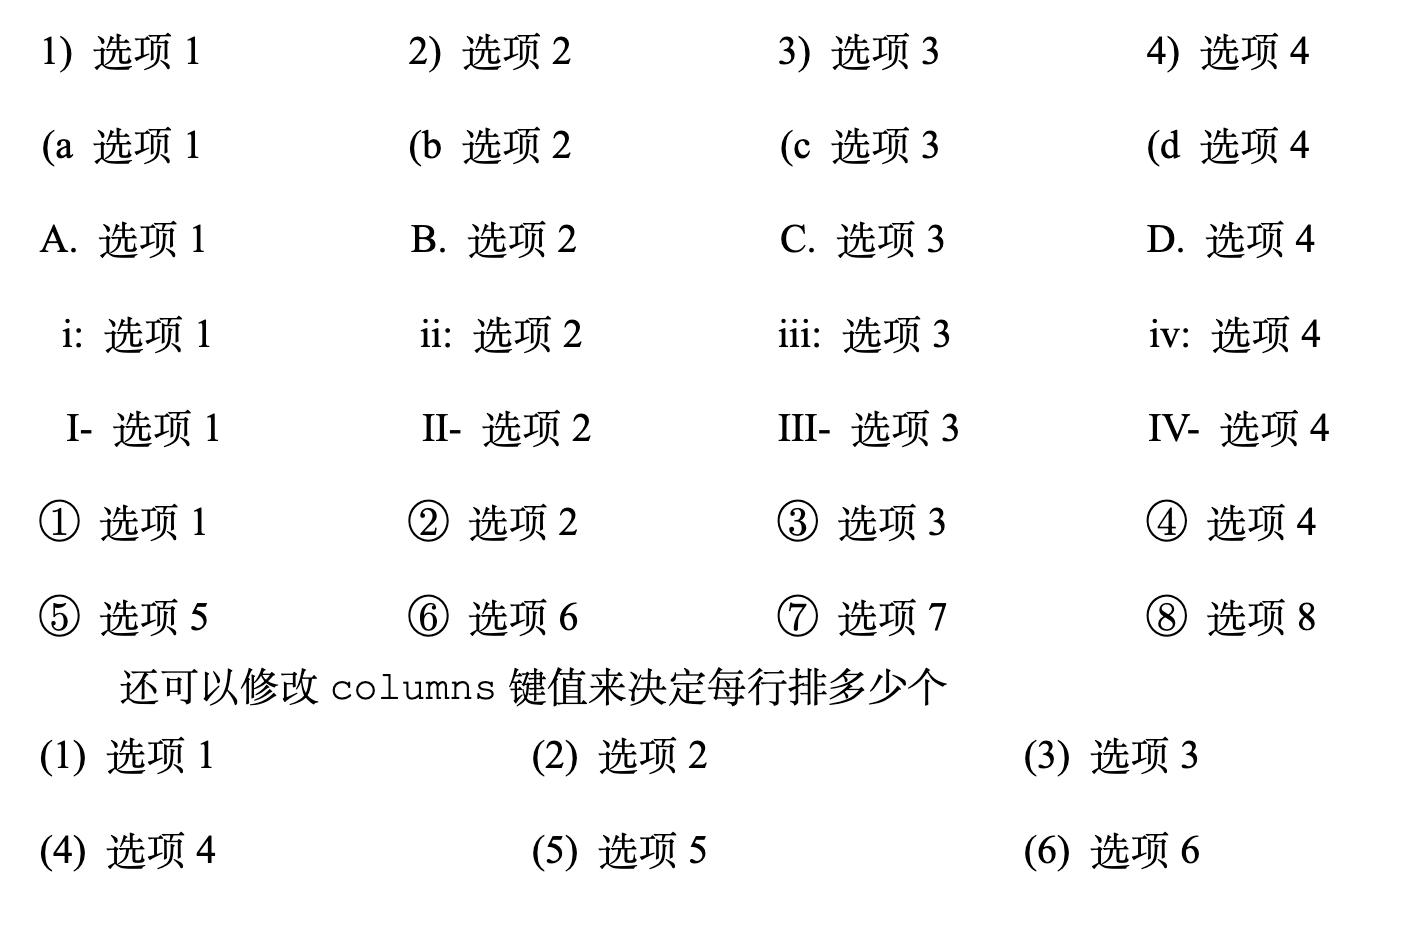
\includegraphics[width = 0.9\textwidth]{choices环境.png}
  \caption{\env{choices} 环境示例}
  \label{figure:choices环境示例}
\end{figure}
% 宏包依赖情况
% !TeX root = ../CCNUthesis.tex

\section{宏包依赖情况}

使用不同编译方式、指定不同选项,会导致宏包依赖情况有所不同。
具体如下:
\begin{itemize}
  \item 在任何情况下,本模板都会\emph{显式}调用以下宏包
    (或文档类):
    \begin{itemize}
      \item \pkg{l3keys2e},用于扩展 \LaTeX3 编程环境。它们属于 \pkg{l3packages} 宏集。
      \item \cls{ctexbook},提供中文排版的通用框架。属于 \CTeX{} 宏集 。
      \item \pkg{geometry},用于调整页面尺寸。
      \item \pkg{fancyhdr},处理页眉页脚。
      \item \pkg{footmisc},处理脚注。
      \item \pkg{graphicx},提供图形插入的接口。
      \item \pkg{caption},用于设置题注。
      \item \pkg{fontspec},设置字体及字号。
      \item \pkg{tikzpagenodes},封面、扉页元素定位。
      \item \pkg{tabularray},表格宏包。
      \item \pkg{calc},提供 \tn{settototalheight} 等命令处理封面下划线。
      \item \pkg{etoolbox},给命令环境打补丁。
      \item \pkg{amsthm}、\pkg{thmtools},提供定理类环境设置接口。
      \item \pkg{xeCJKfntef},提供个人信息的下划线。
      \item \pkg{enumitem},列表环境相关设置。
      \item \pkg{tocloft},目录修改。
      \item \pkg{newtxmath} 和 \pkg{unicode-math},如果 \kvopt{style/font}{newtx} 或 \kvopt{style/font}{times} 则加载前者,其余选项则载入后者。后者对 \LaTeX 的数学排版功能进行了全面扩展。属于 \AmSLaTeX 套件
      \item  \pkg{biblatex},并依赖 \biber{} 程序。参考文献样式由\pkg{biblatex-gb7714-2015} 宏包提供。
      \item \pkg{hyperref},提供交叉引用、超链接、电子书签等功能。
    \end{itemize}
  \item 开启 \kvopt{style/footnote-style}{pifont} 后,会调用
    \pkg{pifont} 宏包。它属于 \pkg{psnfss} 套件。
\end{itemize}

这里只列出了本模板直接调用的宏包。这些宏包自身的调用情况,此处不再具体展开。如有需要,请参阅相关文档。



\section{附录}

% 如何提问
% !TeX root = ../CCNUthesis.tex

\subsection{提问的智慧}

在使用 \LaTeX{} 的过程中,难免会遇到各种各样的问题,那么如何解决这些问题?很关键的一点是学会提问。以下内容选自 \href{https://github.com/ryanhanwu/How-To-Ask-Questions-The-Smart-Way/blob/main/README-zh_CN.md}{《提问的智慧》(简体中文版)}(也非常推荐用户阅读全文,此文不仅仅只对 \LaTeX{} 的使用有帮助,“提问的智慧”可用于方方面面)并结合 \LaTeX{} 做了相应的调整。


\subsubsection{为什么要学会提问}

在黑客的世界里,当您拋出一个技术问题时,最终是否能得到有用的回答,往往取决于您所提问和追问的方式。

现在开源(Open Source)软件已经相当盛行,您通常可以从其他更有经验的用户那里获得与黑客一样好的答案,这是件好事;和黑客相比,用户们往往对那些新手常遇到的问题更宽容一些。尽管如此,以我们在此推荐的方式对待这些有经验的用户通常也是从他们那里获得有用答案的最有效方式。

首先您应该明白,黑客们喜爱有挑战性的问题,或者能激发他们思维的好问题。如果我们并非如此,那我们也不会成为您想询问的对象。如果您给了我们一个值得反复咀嚼玩味的好问题,我们自会对您感激不尽。好问题是激励,是厚礼。好问题可以提高我们的理解力,而且通常会暴露我们以前从没意识到或者思考过的问题。对黑客而言,“好问题!” 是诚挚的大力称赞。

尽管如此,黑客们有着蔑视或傲慢面对简单问题的坏名声,这有时让我们看起来对新手、无知者似乎较有敌意,但其实不是那样的。

我们不讳言我们对那些不愿思考、或者在发问前不做他们该做的事的人的蔑视。那些人是时间杀手 —— 他们只想索取,从不付出,消耗我们可用在更有趣的问题或更值得回答的人身上的时间。我们称这样的人为 失败者(撸瑟) (由于历史原因,我们有时把它拼作 lusers)。

我们意识到许多人只是想使用我们写的软件,他们对学习技术细节没有兴趣。对大多数人而言,电脑只是种工具,是种达到目的的手段而已。他们有自己的生活并且有更要紧的事要做。我们了解这点,也从不指望每个人都对这些让我们着迷的技术问题感兴趣。尽管如此,我们回答问题的风格是指向那些真正对此有兴趣并愿意主动参与解决问题的人,这一点不会变,也不该变。如果连这都变了,我们就是在降低做自己最擅长的事情上的效率。

我们(在很大程度上)是自愿的,从繁忙的生活中抽出时间来解答疑惑,而且时常被提问淹没。所以我们无情地滤掉一些话题,特别是拋弃那些看起来像失败者的家伙,以便更高效地利用时间来回答赢家(winner)的问题。

如果您厌恶我们的态度,高高在上,或过于傲慢,不妨也设身处地想想。我们并没有要求您向我们屈服 —— 事实上,我们大多数人非常乐意与您平等地交流,只要您付出小小努力来满足基本要求,我们就会欢迎您加入我们的文化。但让我们帮助那些不愿意帮助自己的人是没有效率的。无知没有关系,但装白痴就是不行。

所以,您不必在技术上很在行才能吸引我们的注意,但您必须表现出能引导您变得在行的特质 —— 机敏、有想法、善于观察、乐于主动参与解决问题。如果您做不到这些使您与众不同的事情,我们建议您花点钱找家商业公司签个技术支持服务合同,而不是要求黑客个人无偿地帮助您。

如果您决定向我们求助,当然您也不希望被视为失败者,更不愿成为失败者中的一员。能立刻得到快速并有效答案的最好方法,就是像赢家那样提问 —— 聪明、自信、有解决问题的思路,只是偶尔在特定的问题上需要获得一点帮助。

总结来说,为了节约双方的时间,并能够高效地解决您的问题,您需要\emph{学会提问}。


\subsubsection{在提问之前}

在您提问之前,请先做到以下的事情:
\begin{enumerate}
  \item 仔细完整地阅读过 \file{CCNUthesis.pdf} (即此手册)
  \item 完整读过 \href{https://ctan.math.illinois.edu/info/lshort/chinese/lshort-zh-cn.pdf}{lshort-zh-cn},并且在其中进行过相关的查询
  \item 尝试在 \cls{CCNUthesis} 项目主页的 Wiki (\href{https://gitee.com/xkwxdyy/CCNUthesis/wikis/Home}{gitee Wiki} 或 \href{https://github.com/xkwxdyy/CCNUthesis/wikis/Home}{github Wiki} )中找到答案
  \item 尝试在 \cls{CCNUthesis} 项目主页的 issues (\href{https://gitee.com/xkwxdyy/CCNUthesis/issues}{gitee issues} 或 \href{https://github.com/xkwxdyy/CCNUthesis/issues}{github issues} )中找到答案(可以点击“已完成”来查看以往的问题和回答)
  \item 如果是某个命令或环境出问题了,自己检查是否按照规范正确使用该命令或环境,是否少写或多写了括号等等;如果是某宏包的命令或环境,是否通过 \cmd{texdoc} \meta{宏包名} 查看宏包手册来查询命令或环境的具体使用方式
  \item 如果是参考文献出问题了,自己检查
    \begin{enumerate}
      \item \file{.bib} 文件里面的条目是否输入有误,是否漏了西文逗号,是否某个逗号输入了中文的逗号(必须是西文的),参考文献的类型是否有误
      \item 正文中是否按照手册~\ref{para:参考文献引用} 节中的命令正确引用
      \item 是否通过手册~\ref{subsec:编译方式} 节中所说的编译方式正确编译
    \end{enumerate}
  \item 是否去搜索引擎搜索过相应的问题。推荐 \LaTeX{} 的 Stack Exchange 社区网站 \href{https://tex.stackexchange.com/}{LaTeX Stack Exchange}。
\end{enumerate}


\subsubsection{在哪里提问以及如何提问}

如果上述问题自查并没有解决您的问题,那么您可以进行相应的提问了。

首先推荐在 \cls{CCNUthesis} 项目的 issues (\href{https://gitee.com/xkwxdyy/CCNUthesis/issues}{gitee issues} 或 \href{https://github.com/xkwxdyy/CCNUthesis/issues}{github issues} )中新建 issue 进行提问:
  \begin{enumerate}
    \item 使用有意义且描述明确的标题。标题简明扼要地概括出问题。一个好标题范例是\emph{目标 —— 差异}式的描述,许多技术支持组织就是这样做的。在\emph{目标}部分指出是哪一个或哪一组东西有问题,在\emph{差异}部分则描述与期望的行为不一致的地方。比如
      \begin{latexexample}[gobble = 8]
        在v1.2.4版本的 CCNUthesis 模版的正文使用了 $f(x) > 1, 当且仅当 x > 0$ 但是却没有显示中文
      \end{latexexample}
    要比“我公式里怎么没有显示中文啊”的标题要好得多。
    
    编写\emph{目标 —— 差异} 式描述的过程有助于您组织对问题的细致思考。是什么被影响了,只有这个中文还是还有其它部分不能显示?只有版本 1.2.4 无法显示还是以前显示正常但是更新了新版本的模版后显示出问题?是只有我这边出问题了还是我的朋友同学都有这个问题?
    \item 精确地描述问题并言之有物。
      \begin{itemize}
        \item 仔细、清楚地描述您的问题或 Bug 的症状。
        \item 描述问题发生的环境。操作系统,模版的版本,以及在问题出现前是进行了什么操作?比如
          \begin{latexexample}[gobble = 12]
            在输入某代码前还是正常的,但是输入某代码后就编译出错
          \end{latexexample}
        \item 描述在提问前您是怎样去研究和理解这个问题的。您觉得问题出在哪里?您做了什么措施去解决这个问题?
        \item 描述最近做过什么可能相关的硬件或软件变更。有没有换了电脑或更换了编译器
        \item 尽可能地提供一个可以重现这个问题的方法。比如自己检查出某行代码就是问题所在,那么至少提供此行代码让别人能够复现这个问题,从而更好地帮助解决。
      \end{itemize}
  \end{enumerate}

其次就是在模版的 QQ 群里提问(群号:435903068)。但也确保您先进行了自查。具体的细节也和上面在 issue 里提问类似。下面提供几个提问示例:

\begin{latexexample}
  % 编译出错类型问题
  安装的 LaTeX 发行版:TeXLive2022
  电脑型号:macOS
  模版版本:v1.2.4
  问题描述:
    我打算输入一个数学公式,我输入下面这行代码前一些编译都是正常的:
      那么我们就得到了 x = \frac{1}{2}
  报错信息是:
    Missing $ inserted.
    <inserted text>
  可以复现问题的代码:
    \documentclass{CCNUthesis}

    \begin{document}

    那么我们就得到了 x = \frac{1}{2}

    \end{document}
  目的:希望能显示二分之一这个分数
  想法:我已通过手册中所说的方式进行了自查,但仍然没能解决问题,报错说少了一个 $ ,我觉得可能我没有正确地输入这个数学公式。
\end{latexexample}

\begin{latexexample}
  % 不知道如何实现某效果
  安装的 LaTeX 发行版:TeXLive2022
  电脑型号:macOS
  模版版本:v1.2.4
  问题描述:
    - 我打算输入一个数学公式,并且在其中输入中文
    - 我输入下面这行代码
      $f(x) > 1, 当且仅当 x > 1$
      但是里面并没有显示出“当且仅当”四个字
  可以复现问题的代码:
    \documentclass{CCNUthesis}

    \begin{document}

    $f(x) > 1, 当且仅当 x > 1$

    \end{document}
  目的:我希望能够显示出“当且仅当”四个字
  想法:我已通过手册中所说的方式进行了自查,但仍然没能解决问题,我觉得缺少某个命令来输出这个公式中的中文,但我不知道是什么
\end{latexexample}

\begin{latexexample}
  % 格式更改需求
  安装的 LaTeX 发行版:TeXLive2022
  电脑型号:macOS
  模版版本:v1.2.4
  格式现状描述:
    页眉的线距离下方的间距有点窄
  格式需求:
    指导老师说要我把这段距离变大
  可以复现问题的代码:
    \documentclass[type = master]{CCNUthesis}
    
    \ccnusetup{
      style = {
        headline = thin
      }
    }
    \begin{document}

    测试

    \end{document}
  想法:我已通过手册中所说的方式进行了自查,但仍然不知道如何调整这个距离,希望能够编写一个键值来控制这段距离
\end{latexexample}

将三个例子概括出模版:

\begin{latexexample}
  % 编译出错类型问题
  安装的 LaTeX 发行版:
  电脑型号:
  模版版本:v
  问题描述:
  报错信息是:
  可以复现问题的代码:
  目的:
  自己的想法:
\end{latexexample}

\begin{latexexample}
  % 不知道如何实现某效果
  安装的 LaTeX 发行版:
  电脑型号:
  模版版本:v
  问题描述:
  可以复现问题的代码:
  目的:
  想法:
\end{latexexample}

\begin{latexexample}
  % 格式更改需求
  安装的 LaTeX 发行版:
  电脑型号:
  模版版本:v
  格式现状描述:
  格式需求:
  可以复现问题的代码:
  想法:
\end{latexexample}

对于“不知道如何实现某效果”和“格式更改需求”,如果用户无法通过文字准确描述的话,请用纸笔将想要的效果画出来并提供越详细越好的说明。

无论是哪种情况,也可以顺便提供电脑的相应报错\emph{截图},但\textcolor{red}{\emph{请不要用手机对电脑拍照}}。
% 参考文献的类型示例
% !TeX root = ../CCNUthesis-doc.tex

\subsection{参考文献的类型示例} \label{subsec:参考文献的类型示例}

注意:数据中的引用词(@xxx{<引用词>, ...})不允许出现空格!一般推荐的结构为“作者+年份+标题(或部分)”,比如“李晓东1999气候学研究”

以下文献绝大部分来源于 \parencite{本科生院毕业论文注释与参考文献著录格式}。

\subsubsection{期刊文献}

\begin{latexexample}
  @article{李晓东1999气候学研究,
    author          = {李晓东 and 张庆红 and 叶瑾琳},
    title           = {气候学研究的若干理论问题},
    journaltitle    = {北京大学学报:自然科学版},
    year            = {1999},
    volume          = {35},
    number          = {1},
    pages           = {101-106}
  }

  @article{Ahn1993Comparativelinkage,
    author          = {Steven Ahn and Steven D. Tanksley},
    title           = {Comparative linkage maps of the rice and maize genomes},
    journaltitle    = {Proceedings of the National Academy of Sciences of the United States of America},
    year            = {1993},
    volume          = {90},
    pages           = {7980-7984}
  }
\end{latexexample}


\subsubsection{杂志(报纸)文献}

\begin{latexexample}
  @newspaper{丁文祥2000数字革命与竞争国际化,
    author          = {丁文祥},
    title           = {数字革命与竞争国际化},
    journaltitle    = {中国青年报},
    date            = {2000-11-20},
    number          = {15}
  }
\end{latexexample}


\subsubsection{会议论文集}

\begin{latexexample}
  @proceedings{邱泽奇1996当代中国社会结构的过程,  
    author       = {邱泽奇},
    title        = {建构与分化:当代中国社会结构的过程},
    publisher    = {中国社会学纪念费孝通教授学术活动 60 周年学术讨论会},
    year         = {1996},
    address      = {北京}
  }

  @proceedings{雷光春2012综合湿地管理,
    author          = {雷光春},
    title           = {综合湿地管理:综合湿地管理国际研讨会论文集},
    location        = {北京},
    publisher       = {海洋出版社},
    year            = {2012},
  }

  @proceedings{zhang1994Molecularmarkerbased,  
    author       = {Zhang, Q and Gao, Y J and Yang, S H and Ragab, R},
    title        = {Molecular marker-based analysis of heterosis in hybrid rice},
    eventtitle   = {Abstract, 7th Annual Meeting of the Rockefeller Foundation's International Program on Rice Biotechnology},
    year         = {1994},
    address      = {Bali, Indonesia},
  }
\end{latexexample}


\subsubsection{会议论文}

\begin{latexexample}
  @inproceedings{邱泽奇1998当代中国社会结构的过程,
    author          = {邱泽奇},
    title           = {建构与分化:当代中国社会结构的过程},
    editor          = {潘乃谷 and 马戎},
    editortype      = {editor},
    booktitle       = {社区研究与社会发展},
    eventtitle      = {中国社会学纪念费孝通教授学术活动 60 周年学术讨论会},
    address         = {北京},
    eventdate       = {1996},
    location        = {天津},
    year            = {1998},
    publisher       = {天津农业科技术出版社},
    pages           = {1-10}
  }
\end{latexexample}


\subsubsection{普通图书}

\begin{latexexample}
  @book{马克思1995马克思恩格斯选集,
    title        = {马克思恩格斯选集(第1卷)},
    location     = {北京},
    publisher    = {人民出版社},
    year         = {1995},
    pages        = {22-23},
  }

  @book{昂温1988外国出版史,
    author       = {{昂温, G} and {昂温, PS}},
    title        = {外国出版史},
    translator   = {陈生铮},
    location     = {北京},
    publisher    = {中国书籍出版社},
    year         = {1988},
  }

  @book{Foth1984Fundamentalsofsoilscience,
    author       = {Henry D. Foth},
    title        = {Fundamentals of soil science},
    edition      = {7},
    location     = {New York},
    publisher    = {John Wiley & Sons},
    year         = {1984},
    pages        = {151-159},
  }
\end{latexexample}


\subsubsection{专著章节或文集}

\begin{latexexample}
  @inbook{杨国枢1995中国人对现代化的反应,
    author       = {杨国枢},
    title        = {中国人对现代化的反应:心理学的观点},
    editor       = {乔健},
    editortype   = {editor},
    booktitle    = {中国人的观念与行为},
    location     = {天津},
    publisher    = {天津人民出版社},
    year         = {1995},
    pages        = {209-239},
  }

  @inbook{Morison1987Intercellular,
    author       = {James I L Morison},
    title        = {Intercellular $\mathrm{CO}_2$ concentration and stomatal responses to $\mathrm{CO}_2$},
    editor       = {Eduardo Zeiger and Eduardo Zeiger and Eduardo Zeiger and Eduardo Zeiger},
    editortype   = {editor},
    booktitle    = {Stomatal Function},
    location     = {Stanford},
    publisher    = {Stanford University Press},
    year         = {1987},
    pages        = {229-251}
  }
\end{latexexample}


\subsubsection{硕士学位论文}

\begin{latexexample}
  @mastersthesis{徐秀英2013家庭教育对低年级小学生语文学习习惯的影响,
    author       = {徐秀英},
    title        = {家庭教育对低年级小学生语文学习习惯的影响及对策研究},
    location     = {武汉},
    institution  = {华中师范大学},
    year         = {2013}
  }

  @mastersthesis{Aldemita1998GeneticEngineeringofrice,
    author       = {Rhodora Romero Aldemita},
    title        = {Genetic Engineering of rice: Agrobacterium tumefaciens-mediatedtransformation of rice and evaluation of a corn pollen-specific promoter using the gusA gene in transgenic rice},
    location     = {West Lafyatte},
    publisher    = {Purdue University},
    year         = {1998}
  }
\end{latexexample}


\subsubsection{博士学位论文}

\begin{latexexample}
  @phdthesis{张志祥1998间断动力系统,
    author       = {张志祥},
    title        = {间断动力系统的随机扰动及其在守恒律方程中的应用},
    location     = {北京},
    institution  = {北京大学},
    year         = {1998}
  }
\end{latexexample}


\subsubsection{专利}

\begin{latexexample}
  % 国别需要放在number里,例子见Kosekrawtype

  @patent{张凯军2012轨道火车及高速轨道火车,
    author       = {张凯军},
    title        = {轨道火车及高速轨道火车紧急安全制动辅助装置},
    number       = {201220158825.2},     
    date         = {2012-04-05}
  }

  @patent{Kosek2002Compiler,
    author       = {Kosek, A and Momose, H and Kawahito, M and Alan Turling},
    title        = {Compiler},
    number       = {US, 828402},     
    date         = {2002-05-25}
  }
\end{latexexample}


\subsubsection{技术标准}

\begin{latexexample}
  @standard{文献编写1986文献编写规则,
    author       = {全国文献工作标准化技术委员会第六分委员会},
    title        = {GB 6447-86. 文献编写规则},
    location     = {北京},
    publisher    = {中国标准出版社},
    year         = {1986}
  }
\end{latexexample}


\subsubsection{报告}

\begin{latexexample}
  @report{国防白皮2013,
    author       = {中华人民共和国国务院新闻办公室},
    title        = {国防白皮书:中国武装力量的多样化运用},
    date         = {2013-04-16},
    urldate      = {2014-06-11}
  }

  % 当 author 是个组织的时候使用{}框起来
  % 作用是直接输出而不会被修改格式
  @report{federal1990Guidelinesforbandling,
    author       = {{U.S. Department of Transportation Federal Highway Administration}},
    title        = {Guidelines for bandling excavated acid-producing materials, PB 91-194001},
    location     = {Springfield},
    institution  = {U.S. Department of Commerce National Information Service},
    date         = {1990},
    pages        = {22-23} 
  }

  @report{health1970Factorsregulating,
    author       = {{World Health Organization}},
    title        = {Factors regulating the immune response: report of WHO Scientific Group},
    location     = {Geneva},
    institution  = {WHO},
    year         = {1970},
    pages        = {10-11} 
  }
\end{latexexample}


\subsubsection{电子资源}

\begin{latexexample}
  @article{江向东1998互联网环境,
    author          = {江向东},
    title           = {互联网环境下的信息处理与图书管理系统解决方案},
    usera           = {J},
    journal         = {情报学报},
    number          = {2},
    volume          = {18},
    year            = {1998},
    pages           = {4},
    urldate         = {2000-01-18},
    url             = {http://www.chinainfo.gov.cn/periodical/gbxb/gbxb99/gbxb990203}
  }
  @online{萧钮2001出版业信息化迈入快车道,
    author          = {萧钮},
    title           = {出版业信息化迈入快车道},
    year            = {2001-12-19},
    urldate         = {2002-04-15},
    url             = {http://www.creader.com/news/20011219/200112190019.html}
  }
  @online{Dublin2012,
    title           = {Dublin core metadata element set: version 1.1},
    year            = {2012-06-14},
    urldate         = {2014-06-11},
    url             = {http://dublincore.org/documents/dees/}
  }
\end{latexexample}



\section{问题解答}

% 为何使用 LaTeX?
% !TeX root = ../CCNUthesis.tex

\subsection{为什么要用 \LaTeX{}?}

以下主要部分来自 \href{https://ctan.math.illinois.edu/info/lshort/chinese/lshort-zh-cn.pdf}{lshort-zh-cn} 的 1.1.3 \LaTeX{} 的优缺点。

经常有人喜欢对比 \LaTeX{} 和以 Microsoft Office Word 为代表的“所见即所得”(What You See Is What You Get)字处理工具。这种对比是没有意义的,因为 \TeX{} 是一个排版引擎,\LaTeX{} 是其封装,而 Word 是字处理工具。二者的设计目标不一致,也各自有自己的适用范围。

不过,这里仍旧总结 \LaTeX{} 的一些优点:
\begin{itemize}
  \item 具有专业的排版输出能力,产生的文档看上去就像“印刷品”一样。
  \item 具有方便而强大的数学公式排版能力,无出其右者。
  \item 绝大多数时候,用户只需专注于一些组织文档结构的基础命令,无需(或很少)操心文档的版面设计。\emph{这本质上体现了 \LaTeX{} 最重要的思想之一:内容与样式分离(更多关于内容与样式分离的内容可以看 \href{https://liam.page/2019/03/18/separation-of-content-and-presentation/}{到底什么是「内容与样式分离」}一文)},也是 \cls{CCNUthesis} 模版的最基本但也最重要的处理思想:格式由开发者处理,用户只需要关注内容。
  \item 很容易生成复杂的专业排版元素,如脚注、交叉引用、参考文献、目录等。
  \item 强大的可扩展性。世界各地的人开发了数以千计的 \LaTeX{} 宏包用于补充和扩展 \LaTeX{} 的功能。
  \item 能够促使用户写出结构良好的文档——而这也是 \LaTeX{} 存在的初衷。
  \item \LaTeX{} 和 \TeX{} 及相关软件是跨平台、免费、开源的。无论用户使用的是 Windows,macOS(OS X),GNU/Linux 还是 FreeBSD 等操作系统,都能轻松获得和使用这一强大的排版工具,并且获得稳定的输出。
\end{itemize}
% 如何在终端使用 \LaTeX ?
% !TeX root = ../CCNUthesis.tex

\subsection{如何在终端使用 \LaTeX ?}

参考 \href{https://github.com/syvshc}{syvshc}(\cls{hithesis} 和 \cls{elegantbook} 的维护者之一) 的博客 \href{https://syvshc.github.io/2022-03-06-latex-terminal-compiling}{如何在终端使用 LaTeX ?} 和 \href{https://syvshc.github.io/2022-04-20-latex-tutorial/}{latex-tutorial}
% 如何配置 VSCode
% !TeX root = ../CCNUthesis.tex

\subsection{如何安装、配置和使用 VS Code}   \label{subsec:VScode}

参考 \href{https://gitee.com/xkwxdyy/CCNUthesis/wikis/VScode%E7%9A%84%E5%AE%89%E8%A3%85%E9%85%8D%E7%BD%AE%E5%92%8C%E4%BD%BF%E7%94%A8}{如何安装、配置和使用 VS Code}
% 如何配置 PDF 阅读器
% !TeX root = ../CCNUthesis.tex

\subsection{如何配置外置 PDF 阅读器}

参考 \href{https://gitee.com/xkwxdyy/CCNUthesis/wikis/%E5%AE%89%E8%A3%85%E9%85%8D%E7%BD%AE%E5%A4%96%E7%BD%AEPDF%E9%98%85%E8%AF%BB%E5%99%A8}{如何配置外置 PDF 阅读器}
% 如何更新宏包
% !TeX root = ../CCNUthesis.tex

\subsection{如何更新宏包}

\begin{itemize}
  \item Windows用户,在控制台 cmd 中输入
  
  \begin{shellexample}[gobble = 4]
    tlmgr update --all --self
  \end{shellexample}
  
  回车,然后等待更新宏包完成再使用
  
  \item Mac用户,在终端(terminal)输入
  
  \begin{shellexample}[gobble = 4]
    tlmgr update --all --self
  \end{shellexample}
  
  回车,如果提示``No permission'',输入
  
  \begin{shellexample}[gobble = 4]
    sudotlmgr update --all --self
  \end{shellexample}
  
  然后输入管理员密码,回车即可
\end{itemize}


\subsubsection{关于 \TeXLive 包管理器 \cmd{tlmgr} 的其他功能}

关于一些简短的功能,可以查看 \href{http://mirrors.ctan.org/info/tlmgrbasics/doc/tlmgr.pdf}{tlmgrBasics},syvshc 做了部分内容的翻译,见~\href{http://mirrors.ctan.org/info/tlmgr-intro-zh-cn/tlmgr-intro-zh-cn.pdf}{tlmgr-intro-zh-cn}。

更完整的使用说明可以看~\href{https://www.tug.org/texlive/doc/tlmgr.html}{full document for tlmgr}。


\subsubsection{如果升级到一半意外终止了更新,如何继续}

当使用 \cmd{tlmgr} 升级宏包到一半时因为意外终止, 运行下面的命令来继续没有完成的升级:

\begin{shellexample}
  tlmgr update –reinstall-forcibly-removed –all
\end{shellexample}


\subsubsection{windows用户:如果更新时,不小心点了一下 cmd 窗口,宏包更新暂停了怎么办}

重新点一下窗口,然后回车
% 为什么不推荐使用 CTeX 套装 了?
% !TeX root = ../CCNUthesis.tex

\subsection{关于 \CTeX 套装的相关问题}


\subsubsection{为什么不推荐安装 \CTeX 套装了?}

\CTeX 套装最早是由中科院 Leo Wu(吴凌云)研究员开发、维护和发布的 \TeX{} 发行版,它是应当时中文配置困难的背景(CCT、CJK 等)而诞生的,而现在的中文支持技术(xeCJK等)配置已非常简单;

\CTeX 套装自 2012 年 3 月 22 日发行 2.9.2.164 版本后,至今未更新,已不能适应当前 TeX 中文技术的发展,引用 \CTeX 套装的开发者之一刘海洋的话:
\begin{latexexample}
  CTeX 已经完成了它的历史使命。
\end{latexexample}


\subsubsection{\CTeX 套装的问题}

\begin{itemize}
  \item 最主要的bug是:在一定条件下,\CTeX 套装在安装时会抹掉系统环境变量,造成一定损失(有可能会引起一些程序不能运行或者是运行出错(只是有可能,具体视情况而定,但是这个可能性就已经是个问题了))
  \item 版本落后:\CTeX 套装的「最新版本」发布于 2012 年 3 月。除了新增的功能用不上、已经修复的 bug 避免不了,还可能遇到
    \begin{itemize}
      \item 提问不易收到回答(因为社区活跃用户中 \CTeX 套装的比例极低,帮忙解答时复现问题的成本高),
      \item 与 \CTeX 套装有关的正确有效的网络资源少(英文资源几乎为零)等等弊端。
    \end{itemize}
  \item 乱码问题,2017 届使用 \CTeX 套装模版的同学毕业论文查重结果普遍出现乱码现象
  \item 中英文混排问题、数学式和中文混排的空格处理比较麻烦
  \item 系统问题。不支持 mac 系统,虚拟机的安装配置或更换电脑增加了用户的学习成本。
\end{itemize}


\subsubsection{关于 \CTeX 套装我想说的}

\begin{itemize}
  \item 我们不再推荐 \CTeX 套装,并不是想否定它在早些年的“丰功伟绩”,只是它的使命在现代 \LaTeX 使用中已经基本结束了(除非你要投稿一些中文核心期刊,要求得安装,那没办法),它更像是一个 \LaTeX 在中国传播过程中的一个开拓者,它的作用是绝对不可磨灭的,但我相信,如果它有自己的想法的话,也会希望后人能够用更好更高效的方式使用 \LaTeX
  
  \item 分享一段话
    \begin{latexexample}[gobble = 6]
      另一方面,从用户社区的问答中可以观察到,一些 \CTeX 套装的老用户,其 LaTeX 的使用水平尚有很大进步空间,少数用户一直在以不推荐、甚至绝对错误的方式编写 tex 文件。这里有必要给新用户提个醒:你身边的老用户,不一定比网线另一端的老用户,更熟练、更专业;看「独家祖传文档」,不如看更方便获取的、更正式的文档。
      —— 2018年,为什么不推荐使用 CTeX 套装了(https://zhuanlan.zhihu.com/p/45174503)
    \end{latexexample}
  
    \CTeX 套装的很多使用方式在现代 \LaTeX 使用观点看是不推荐甚至是错误的,例子就是邓国泰老师在模版培训提到的一些使用,我列举了部分和现代 \LaTeX 使用有较大出入的部分进行讲解:
  
  \item 如果因为某些不可抗力的原因一定要安装 \CTeX 套装
    \begin{itemize}
      \item 请\emph{备份好环境变量}(自行查找资料)
      \item 并尝试更新全部宏包,但编译出偏差须自行负责:
        \begin{enumerate}
          \item 运行cmd,输入mpm命令
          \item 进入 Repository 菜单 → 选择 Change Package Repository → 选择 Packages shall be installed from the Internet → 选择一个可用的地址
          \item 更新 CTeX 宏包。
        \end{enumerate}
    \end{itemize}
    
  \item 如果没有备份环境变量的结果可以看看这个 \href{https://github.com/CTeX-DEV/CTeX/issues/19}{issue} 来了解后果。
\end{itemize}


更多细节可以参考下面的几篇:

\begin{itemize}
  \item \href{https://zhuanlan.zhihu.com/p/45174503}{[LaTeX 发行版] 2018年,为什么不推荐使用 \CTeX 套装了}
  \item \href{https://zhuanlan.zhihu.com/p/73304856}{[LaTeX 期刊模板] els-cas-templates 不支持 \CTeX 套装}
  \item \href{https://zhuanlan.zhihu.com/p/112637535}{[LaTeX 期刊模板] siamart 不支持 \CTeX 套装}
  \item \href{https://tieba.baidu.com/p/2665622350}{不推荐 \CTeX 套装作为入门}
\end{itemize}


\subsubsection{如果安装了 \CTeX 套装怎么办?}

先明确你要使用哪个模版,旧模版还是 \cls{CCNUthesis},二者不兼容。

如果要用旧模版,那么一切使用和问题请找邓国泰老师。

如果确定要使用 \cls{CCNUthesis},卸载掉 \CTeX 套装,然后跟着[install-latex-guide-zh-cn](https://gitee.com/OsbertWang/install-latex-guide-zh-cn/releases) 文档正确安装 \TeXLive 。


但是卸载 \CTeX 套装并安装了 `TeX Live`后,用户可能会发现无法编译参考文献(但是正常的 `xelatex` 编译是可行的),这个时候参考
\href{https://gitee.com/xkwxdyy/CCNUthesis/wikis/%E5%8D%B8%E8%BD%BD%E4%BA%86CTeX%E5%A5%97%E8%A3%85%E5%AE%89%E8%A3%85%E4%BA%86TeXLive%E5%8D%B4%E6%97%A0%E6%B3%95%E7%BC%96%E8%AF%91%E5%8F%82%E8%80%83%E6%96%87%E7%8C%AE}{卸载了 CTeX 套装,安装了 TeX Live 却无法编译参考文献怎么办?}


\subsubsection{\cls{CCNUthesis} 模版和 \CTeX 套装写的旧模版相比有什么优点}

\CTeX 套装写的旧模版的问题除了上面 \CTeX 套装本身的问题外,还有
\begin{enumerate}
  \item 用户界面的接口设计的不好,有许多不该在正文出现的 \tn{def} 命令(\cls{CCNUthesis} 的用户接口见 \file{main.tex})
  \item 如果去读旧模版的源码会发现一些处理并不当,这些讨论均在 \href{https://gitee.com/xkwxdyy/CCNUthesis/wikis/%E6%97%A7%E6%A8%A1%E7%89%88%E7%9A%84%E9%97%AE%E9%A2%98%E5%92%8C%E6%96%B0%E6%A8%A1%E7%89%88%E7%9A%84%E5%A4%84%E7%90%86}{旧模版的问题和新模版的处理}
\end{enumerate}

\cls{CCNUthesis} 模版的优点概括起来主要有
\begin{enumerate}
  \item Windows, Mac, Linux 平台均可使用
  \item 极大分离了内容和样式,提供了丰富且详细的接口,让用户更专注于内容创作本身,极大提高了用户使用 \LaTeX{} 撰写论文的效率。
  \item 极大地优化了旧模版中的 bug 和一些使用问题,详细见 \href{https://gitee.com/xkwxdyy/CCNUthesis/wikis/%E6%97%A7%E6%A8%A1%E7%89%88%E7%9A%84%E9%97%AE%E9%A2%98%E5%92%8C%E6%96%B0%E6%A8%A1%E7%89%88%E7%9A%84%E5%A4%84%E7%90%86}{旧模版的问题和新模版的处理}
\end{enumerate}
% 参考文献的相关问题
% !TeX root = ../CCNUthesis-doc.tex

\subsection{参考文献的相关问题}

\subsubsection{ bib 文件如何使用}

主要参考 \href{https://ctan.math.illinois.edu/info/lshort/chinese/lshort-zh-cn.pdf}{lshort-zh-cn} 的 6.1.2 节,但在这多说一点,参考文献的数据库(\file{.bib} 文件)中文献条目的获取方式,可以通过 google 学术等搜索文献,然后“导出 bib 格式”,或是用 zotero 等软件管理参考文献进行导出 bib 格式。

但要注意的事,这样的导出方式,经常出现文献的类型不匹配,所以需要自己根据~\ref{subsec:参考文献的类型示例} 节的数据类型自行甄别。


\subsubsection{作者姓氏的多音字问题}

在设置了
\begin{latexexample}
  \ccnusetup{
    style = {
      bib-style = ccnu-bachelor-author-year
    }
  }
\end{latexexample}
后,即此时参考文献的格式为作者-年制,但是有的时候会发现一些中文作者文献的顺序“出乎意料”,比如第一作者为“曾xx”的文献竟然会排在非 Z 开头的文献前,这主要是姓氏的多音字问题,比如“曾”就有“\pinyin{ceng2}”和“\pinyin{zeng1}”两种读音,而默认会取字母靠前的作为读音,就导致了自动把“曾xx”的“曾”作为“\pinyin{ceng2}”进行排序所以才有了上述的结果。

那怎么解决呢?这个时候需要用到 \cmd{key} 域

\begin{latexexample}[emph={key}]
  @book{曾谨言2013量子力学,
    title     = {量子力学: 卷 I},
    author    = {曾谨言},
    year      = {2013},
    publisher = {科学出版社},
    address   = {北京},
    pages     = {1-10},
    edition   = {2},
    key       = {zeng1jin3yan3}
  }
\end{latexexample}

内容就是第一作者名的拼音,用法一看这个示例便知(和 \pkg{xpinyin} 宏包的使用相同)。然后按照正确的参考文献编译方式(因为 \LaTeX 要重新写 \file{.bbl} 文件)重新编译即可获得正确的排序。



% 拓展阅读
% !TeX root = ../CCNUthesis-doc.tex

\section{拓展阅读} \label{sec:拓展阅读}

\begin{itemize}
  \item \href{https://github.com/stone-zeng}{stone-zeng}( \cls{fduthesis} (复旦大学学位论文模板) 开发者和维护者):\href{https://www.bilibili.com/video/BV1RE411W7FS?p=1}{现代LaTeX入门讲座视频} 
  \item \href{https://github.com/zepinglee}{zepinglee}( \cls{thuthesis} (清华大学学位论文模板) 维护者,\cls{ustcthesis} (中科大学位论文模板) 开发者和维护者): \href{https://gitee.com/zepinglee/latex2e-style-guide}{LaTeX2e代码规范} 
  \item \href{https://liam.page/}{liam}( \pkg{xprintlen} , \cls{sduthesis} 和 \cls{mcmthesis} 的开发者):\href{https://liam.page/2019/03/18/separation-of-content-and-presentation/}{到底什么是「内容与样式分离」}
  \item \href{http://liantze.penguinattack.org/index.html}{林莲枝}(马来西亚 TeX 用户组织的首席写手、Overleaf 网站的技术支援人员兼模板开发人员):\href{https://www.bilibili.com/video/BV1r4411o7KJ?spm_id_from=333.999.0.0}{漫谈 LaTeX 排版常见概念误区}
  \item \href{https://github.com/sikouhjw}{sikouhjw}( \cls{gdutthesis} 开发者和维护者): \href{https://sikouhjw.github.io/2020/03/08/2020-03-08-Learn-LaTeX}{关于LaTeX入门的一点东西} 
  \item \href{https://github.com/stone-zeng}{stone-zeng}( \cls{fduthesis} (复旦大学学位论文模板) 开发者和维护者):\href{https://stone-zeng.github.io/2019-07-23-latex-crime-and-punishment/}{回「 LaTeX 的罪与罚 」}
  \item \href{https://zhuanlan.zhihu.com/typography-and-latex/}{muzimuzhi} : \href{https://zhuanlan.zhihu.com/p/43981639}{[LaTeX 指南] 功能性宏包推荐}
  \item \href{https://zhuanlan.zhihu.com/typography-and-latex/}{muzimuzhi} : \href{https://zhuanlan.zhihu.com/p/43938945}{[LaTeX 指南]常用参考文档}
\end{itemize}



% 参与开发
% !TeX root = ../CCNUthesis.tex

\section{参与开发}

\begin{itemize}
  \item 如果您有任何改进意见或者功能需求,欢迎前往 \href{https://github.com/xkwxdyy/CCNUthesis/issues}{github 仓库 issues} 或 \href{https://gitee.com/xkwxdyy/CCNUthesis/issues}{gitee 仓库 issues} 提交 issue
  \item 您也可以发送邮件到 \href{mailto:kangweixia_xdyy@163.com}{我的邮箱}
  \item 欢迎 \cmd{fork} 本项目,提 \cmd{pr} 的形式参与开发
  \item 建议阅读 \href{https://zhuanlan.zhihu.com/typography-and-latex/}{muzimuzhi} 写的 \href{https://github.com/ustctug/ustcthesis/wiki/%E5%8F%82%E4%B8%8E%E5%BC%80%E5%8F%91}{参与开发}
  \item 参考阅读
    \begin{itemize}
      \item \href{https://www.zhihu.com/question/27017364/answer/34932199}{知乎:开发一个 LaTeX 宏包需要多少知识?}
      \item \href{https://zhuanlan.zhihu.com/p/19669122}{The TeXbook 导读:从那头(多图杀猫的)狮子说起}
    \end{itemize}
\end{itemize}



% 关于作者
% !TeX root = ../CCNUthesis-doc.tex

\section{关于模版作者}

我是华中师范大学数学与统计学学院 2017 级数学与应用数学(试验)专业 1705 班夏康玮,2021 级应届毕业生。目前就读于武汉大学基础数学专业。

在我 2021 年写毕业论文的时候使用的就是邓国泰老师 CTeX 套装编写的模版,当时周围的人,包括我自己,在使用的过程中经常遇到一些奇怪的问题,比如莫名的报错,表格中插图问题等等。但是当时的我只能算个 \LaTeX{} 的半吊子,在大二的时候磕磕绊绊学了一点点 \LaTeX{},不过主要学的是数学公式那一块,其它方面也没怎么涉及,最终也没能够解决模版的问题。

但是在那个时候我就萌发了要写新模版的想法,可是当时能力不够,且重心放在论文的内容上,于是这件事就被我搁置了。

在本科毕业的那个暑假,我花了一个多月“集训” \LaTeX{},并且初步学习了 \LaTeX3。终于在 2022 年的 2 月份,基于 \cls{fduthesis},我开始开发 \cls{CCNUthesis},因为时间紧张,当时就是在 \cls{fduthesis} 的基础上“缝缝补补”,初步实现了邓国泰老师的本科旧模版的效果。

在给 2018 级使用的过程中,也不断出现新问题,新需求,但是在当时只能是临时缝补,因为要做大改动的话,一些 \LaTeX{} 接触少的用户会比较难调整。

终于在 2018 级交完终稿之后,我开始对本科模版的代码进行了几乎整个的推翻重构,并且在使用过程中出现的一些有分歧的需求控制做成了键值控制。同时也在 2022 年 6 月初基本完成了硕博模版的开发工作。

目前模版的主要维护者是我本人。但在开发过程中离不开很多人的帮助:
\begin{itemize}
  \item 感谢 \href{https://github.com/syvshc}{syvshc} 帮忙开发了西文字体的部分
  \item 感谢 \href{https://github.com/stone-zeng}{stone-zeng} 开发的 \cls{fduthesis} (模版开发初期的代码框架是基于 \cls{fduthesis})
  \item 感谢 \href{https://github.com/zepinglee}{zepinglee} 在 \cls{CCNUthesis} 开发过程中提供的帮助。
\end{itemize}

俗话说,投资效率是最好的投资。如果您觉得本模版对您有帮助,提高了您写论文的效率,不妨通过图~\ref{figure:alipay-wechat} 小额赞助我一下,这会支持我继续维护和完善模版。

\begin{figure}[htbp]
  \centering
  
\includegraphics[width = \textwidth]{夏大鱼羊支付宝微信收款码.png}
  \caption{支付宝和微信收款码}
  \label{figure:alipay-wechat}
\end{figure}



\section{CCNUthesis: TODO}

\begin{itemize}
  \item 手册本身
    \begin{itemize}
      \item 参考文献
    \end{itemize}
  \item wiki
    \begin{itemize}
      \item 问题解决
        \begin{itemize}
          \item 标题中一些宏如果报错:\tn{texorpdfstring}
        \end{itemize}
      \item 学习其它模版的 wiki
      \item 
        \begin{itemize}
          \item VScode
            \begin{itemize}
              \item 左下角是x怎么办
            \end{itemize}
        \end{itemize}
      \item 提供一些示例
        \begin{itemize}
          \item tabularray
          \item physicx
          \item fixdif
          \item choices
        \end{itemize}
    \end{itemize}
  \item 重新整理 issue 的模版
  \item 学习其它论文模版的处理
    \begin{itemize}
      \item thuthesis
      \item sjtuthesis
      \item ucasthesis
      \item ustcthesis
      \item cquthesis
      \item njuthesis
      \item hithesis
    \end{itemize}
  \item 录制新的讲解视频
\end{itemize}

% 参考文献
\printbibliography



\end{document}